% !TEX root = ../Thesis.tex
\chapter{Calibration of the Soft Muon Tagger for 2012 ATLAS Data} \label{prt:Calibration}

High-energy physics relies heavily on the use of simulated data to inform the development of analysis techniques. It is thus paramount that the simulation reflect nature as closely as possible. However the simulation does not accurately predict conditions within the detector and the effects on the muon reconstruction and the quality of the fit between the inner detector tracks and muon spectrometer tracks which is represented in the \xsm. Instead the difference between simulation and data is quantified and taken into account. This process is known as calibration. In the case of the muon reconstruction method and the \xsm\ tagger it is important that the difference in efficiency between MC and data be accounted for. This is done by constructing a scale factor, defined in this case by:

\begin{equation}
  \kappa_{\textrm{\xsm}} = \frac{\epsilon_{\xsm}^{\textrm{Data}}}{\epsilon_{\xsm}^{\textrm{MC}}}
\end{equation}

One of the advantages of using the \xsm\ tagger over other forms of tagging is that the presence of a jet is not required to measure the \xsm\ of a muon. This means that the calibration can be performed on a isolated muons such as those from $\jpsi \rightarrow \mu\mu$ or $Z\rightarrow\mu\mu$ using the so called tag and probe method. This calibration relies on muons with low \pt\ from \jpsi\ decays. As the \xsm\ is a characteristic of combined and therefore reconstructed muons, 

The tag and probe method used in this calibration is defined as follows. One reconstructed combined muon is designated as the Tag, this muon must pass a stringent set of cuts implying that this is indeed a muon from a \jpsi. The second muon which is designated as the Probe is constructed from an inner detector (ID) only. To ensure that the Probe is the second muon from the \jpsi\ decay, the invariant mass of the combined tag and probe system is required to be within a mass window centered around the true \jpsi\ mass. The complete selection used in the calibration is detailed in Section~\ref{sec:CalibrationSelection}. These Probes are then used to measure the reconstruction efficiency and the \xsm\ tagger efficiency as described in Sections~\ref{sec:CalibrationFitting} and \ref{sec:CalibrationEfficiencies}.

The tag and probe method used here is based on a previous calibration of the \xsm\ tagger performed on 2011 ATLAS collision data outlined in %CITE OLD CALIBRATION NOTE.
This analysis differs from the 2011 calibration in several ways these will be highlighted and explained.

\subsection{Software, Collision Data and Simulated samples}
The tag and probe method used here was implemented using the \textsc{ROOT} analysis framework. 

The calibration was performed on a dataset made of those luminosity blocks selected by the recommended standard Good Runs List (GRL) which corresponds to all $pp$ collision periods in 2012. The GRL selects only those luminosity blocks where detector conditions are appropriate for physics data-taking. This includes all relevant detector components being operational and that stable beam conditions have been achieved.
The datasets are part of the 2013 summer reprocessing (processing tag p1328) corresponding to data taken in periods A through to L, excluding periods F and J. 

The efficiency scale factor is measured against a sample containing almost 10 million $\jpsi\rightarrow\mu\mu$ events. At event generation filters are applied so the sample only contains events where both muons have a transverse momentum of at least 4 GeV and they must lie within the pseudo-rapidity range $|\eta|<2.5$. This selection matches the object selection used by most analyses as recommended by the Muon Combined Performance (MCP) group. 

\section{Tag and Probe Selection} \label{sec:CalibrationSelection}

A tag and probe method was chosen to measure the efficiency of muon reconstruction and the \xsm\ tagger. The tag and probe method allows for the measurement of the performance of selection criteria or algorithms by exploiting well known decays. By creating a sample of objects, in this case muons, on which to apply the aforementioned selection criteria, it is possible to study these algorithms.

The muon reconstruction algorithm examines various Inner Detector (ID)tracks and Muon Spectrometer (MS) tracks and makes a determination as to whether said track is produced by muon or not. To measure the performance of the muon reconstruction algorithm a sample of ID tracks which originate from the \jpsi\ decay and are thus very likely to be a real muon is constructed. This is done in the following way:

First, require the presence of a combined \staco\ muon which passes a very stringent selection. This strongly implies that this is a real muon and thus is labelled as the Tag. Additionally a very loose selection is applied to all ID tracks. These are known as candidate Probes. Pairs of tag and probes are then formed by requiring that the combined invariant mass lie within a \jpsi\ mass window and the pair pass additional pairing cuts. This then implies that the Probe is likely the other muon from the \jpsi\ decay and as such is a suitable test-bed to measure the performance of the muon resconstruction algorithm. Note that all selection criteria are detailed and explained in Section~\ref{sec:CalibrationSelectionCuts}

After selecting a sample of probes the performance of the algorithm is estimated by measuring the proportion of probe candidates which are selected by the algorithm. In other words the performance is estimated by counting the number of muons which are reconstructed given that the ID track is very likely to be a real muon. Probes which are reconstructed into combined \staco\ muons are labelled as muon probes. The performance of the \xsm\ tagger is estimated in a similar manner, by measuring the proportion of combined muon probes which pass the SMT selection.

\subsection{Trigger requirements} \label{sec:CalibrationTriggerRequirement}
In order for an event to be included in the analysis it must pass at least one of the trigger chains listed in Appendix~\ref{app:CalibrationTrigger}. For the sake of brevity only the primary trigger (\verb|EF_mu6_Trk_Jpsi_loose|) which contributes the majority of events is described here.

As stated in the trigger name this is an Event Filter trigger which requires the presence of a muon with a momentum of at least 6 GeV and an ID track whos combined invariant mass lies within a \jpsi\ mass window of 2.6 GeV $<m_{\textrm{inv}}<$ 3.6 GeV. This loose mass window contains the entirety of the \jpsi\ peak in all examined $p_{T}$ and $\eta$ ranges as well as additional side bands to allow for background removal. Note the omission of double muon triggers to avoid introducing a bias by specifically selecting events with two good muons. 

Also note that while all triggers are operational in all periods, most are heavily prescaled and the prescale is period dependent. This does not have a first-order effect on the measurement since only ratios are compared between collision data and MC.

\subsection{Selection Cuts} \label{sec:CalibrationSelectionCuts}
The selection criteria for tags, probes, muon probes and SMT muons are listed and detailed below. Note that all cuts are applied on the kinematic properties measured in the ID due to its improved resolution unless it is not possible as in the case of the \xsd\ which is a combined MS and ID property. Also note that all objects must pass a selection criteria collectively refered to as MCP cuts. These are tracking quality cuts which require a certain number of detector elements be active to ensure good tracking. These cuts are listed in 

The muon tag selection criteria are defined in the list below:

\begin{itemize}
  \item MCP cuts
  \item \staco\ collection
  \item Combined muon
  \item $p_{T}>$4 GeV
  \item $|\eta|<$2.5
  \item $|d_{0}|<$0.3 mm and $|z_{0}|<$1.5 mm
  \item $|d_{0}/\sigma_{d_{0}}|<$3 and $|z_{0}/\sigma_{z_{0}}|<$3
  \item Fired at least one of the relevant triggers (see Appendix~\ref{app:CalibrationTrigger})
\end{itemize}

Included are cuts on the muon impact parameter (IP) $d_{0}$ and $z_{0}$. These are defined as the distance of closest approach of the ID track to the primary interaction vertex in the transverse and longitudinal planes, respectively. Additionally cuts on the absolute values of IP significances are also implemented. The signifiance of the impact parameter is defined as $d_{0}/\sigma_{d_{0}}$ where $\sigma{\textrm{IP}}$ is the standard deviation of the impact parameter. These cuts are designed to ensure that the muon selected originates near the primary vertex and thus from a prompt \jpsi\ from the primary collision. Note that non-prompt \jpsi\ can be produced in the decay of $b$ hadrons. Finally note that the tag muon must match the trigger object which selected this event.

The probe selection is a subset of the tag selection and only requires an ID track with $|\eta|<2.5$ and $p_{T}<4$ GeV. The pairing cuts are shown below:

\begin{itemize}
  \item 2 GeV $\leq m_{\textrm{inv}}\leq$ 4 GeV
  \item Probe charge is opposite the tag charge 
  \item 0.4 $<\Delta$R(tag, probe)$<$ 3.5
  \item $\Delta z_{0}$(tag, probe)$<$ 0.2 mm
\end{itemize}

The probe and the tag are required to be fairly well separated to avoid the momentum of the tag from entering the isolation cone of the probe. In the 2011 calibration analysis the track of the tag and the probe are refit to a common vertex and the quality of the refit, expressed by the $\chi^2$ is a part of the pairing criteria. This criteria is present to reduce the effects of pile-up on the measurement, by ensuring both objects have a common origin. Since the data format used for this analysis is a derived form of that used in 2011 it is not possible to perform such a refit. Instead the difference between the $z_{0}$ of the tag and the probe is used.

The \staco\ reconstruction efficiency is not measured by applying the algorithm on the probe collection but rather a probe is said to be a muon probe if it matches a combined muon from the \staco\ collection. This is done by requiring the angular separation between the probe and the \staco\ muon be less than 0.001. Probes which are matched become the numerator of the reconstruction efficiency and the denominator is defined as the number of probes:

\begin{equation*}
  \epsilon = \frac{N_{\textrm{muon probe}}}{N_{\textrm{probe}}}
\end{equation*}

A muon probe is said to be an SMT muon if it passes the following selection, which matches the muon cuts defined in Chapter~\ref{prt:smt_summary}

\begin{itemize}
  \item $|d_{0}|<3$ mm
  \item $|z_{0}\sin(\theta)|<3$
  \item $\xsm/N_{\textrm{dof}}<3.2$
\end{itemize}

Those muon probes which pass the SMT selection are the numerator of the SMT efficiency and the denominator is defined as the number of muon probes:

\begin{equation*}
  \epsilon = \frac{N_{\textrm{SMT}}}{N_{\textrm{muon probe}}}
\end{equation*}

\section{Invariant mass fitting} \label{sec:CalibrationFitting}
The pairing criteria are very effective at selecting \jpsi\ events, however non-\jpsi\ background events are also pass the selection. These include combinatiorial background where the wrong tag and probe pair is constructed and Drell-Yan which appears as a continuum below the \jpsi\ peak.

The number of probes is extracted from a fit to the invariant mass of the dimuon system using a composite function to accomodate for the background and the gaussian-like \jpsi\ peak. 

The invariant mass peak of the \jpsi\ is modelled by a gaussian distribution while the background distribution is modelled by a quadratic. The invariant mass distribution is fit by a sum of the two functions.

To avoid the first-order effects of signal mis-modelling from the fit of the \jpsi\ peak, the yield is obtained from the integral of the measured invariant mass distribution subtracting the background contribution from the integral of the fit to the background. The integration is performed in a window with a width based on the width of the fitted \jpsi\ peak. The integration window marked in Fig.~\ref{fig:CalibrationFittingExample} corresponds to three times the width of the peak or simply $3\sigma$. Additionally note the composite fit line as well as the background-only distribution and the implied signal gaussian peak.

\begin{figure}[htbp]
  \centering
  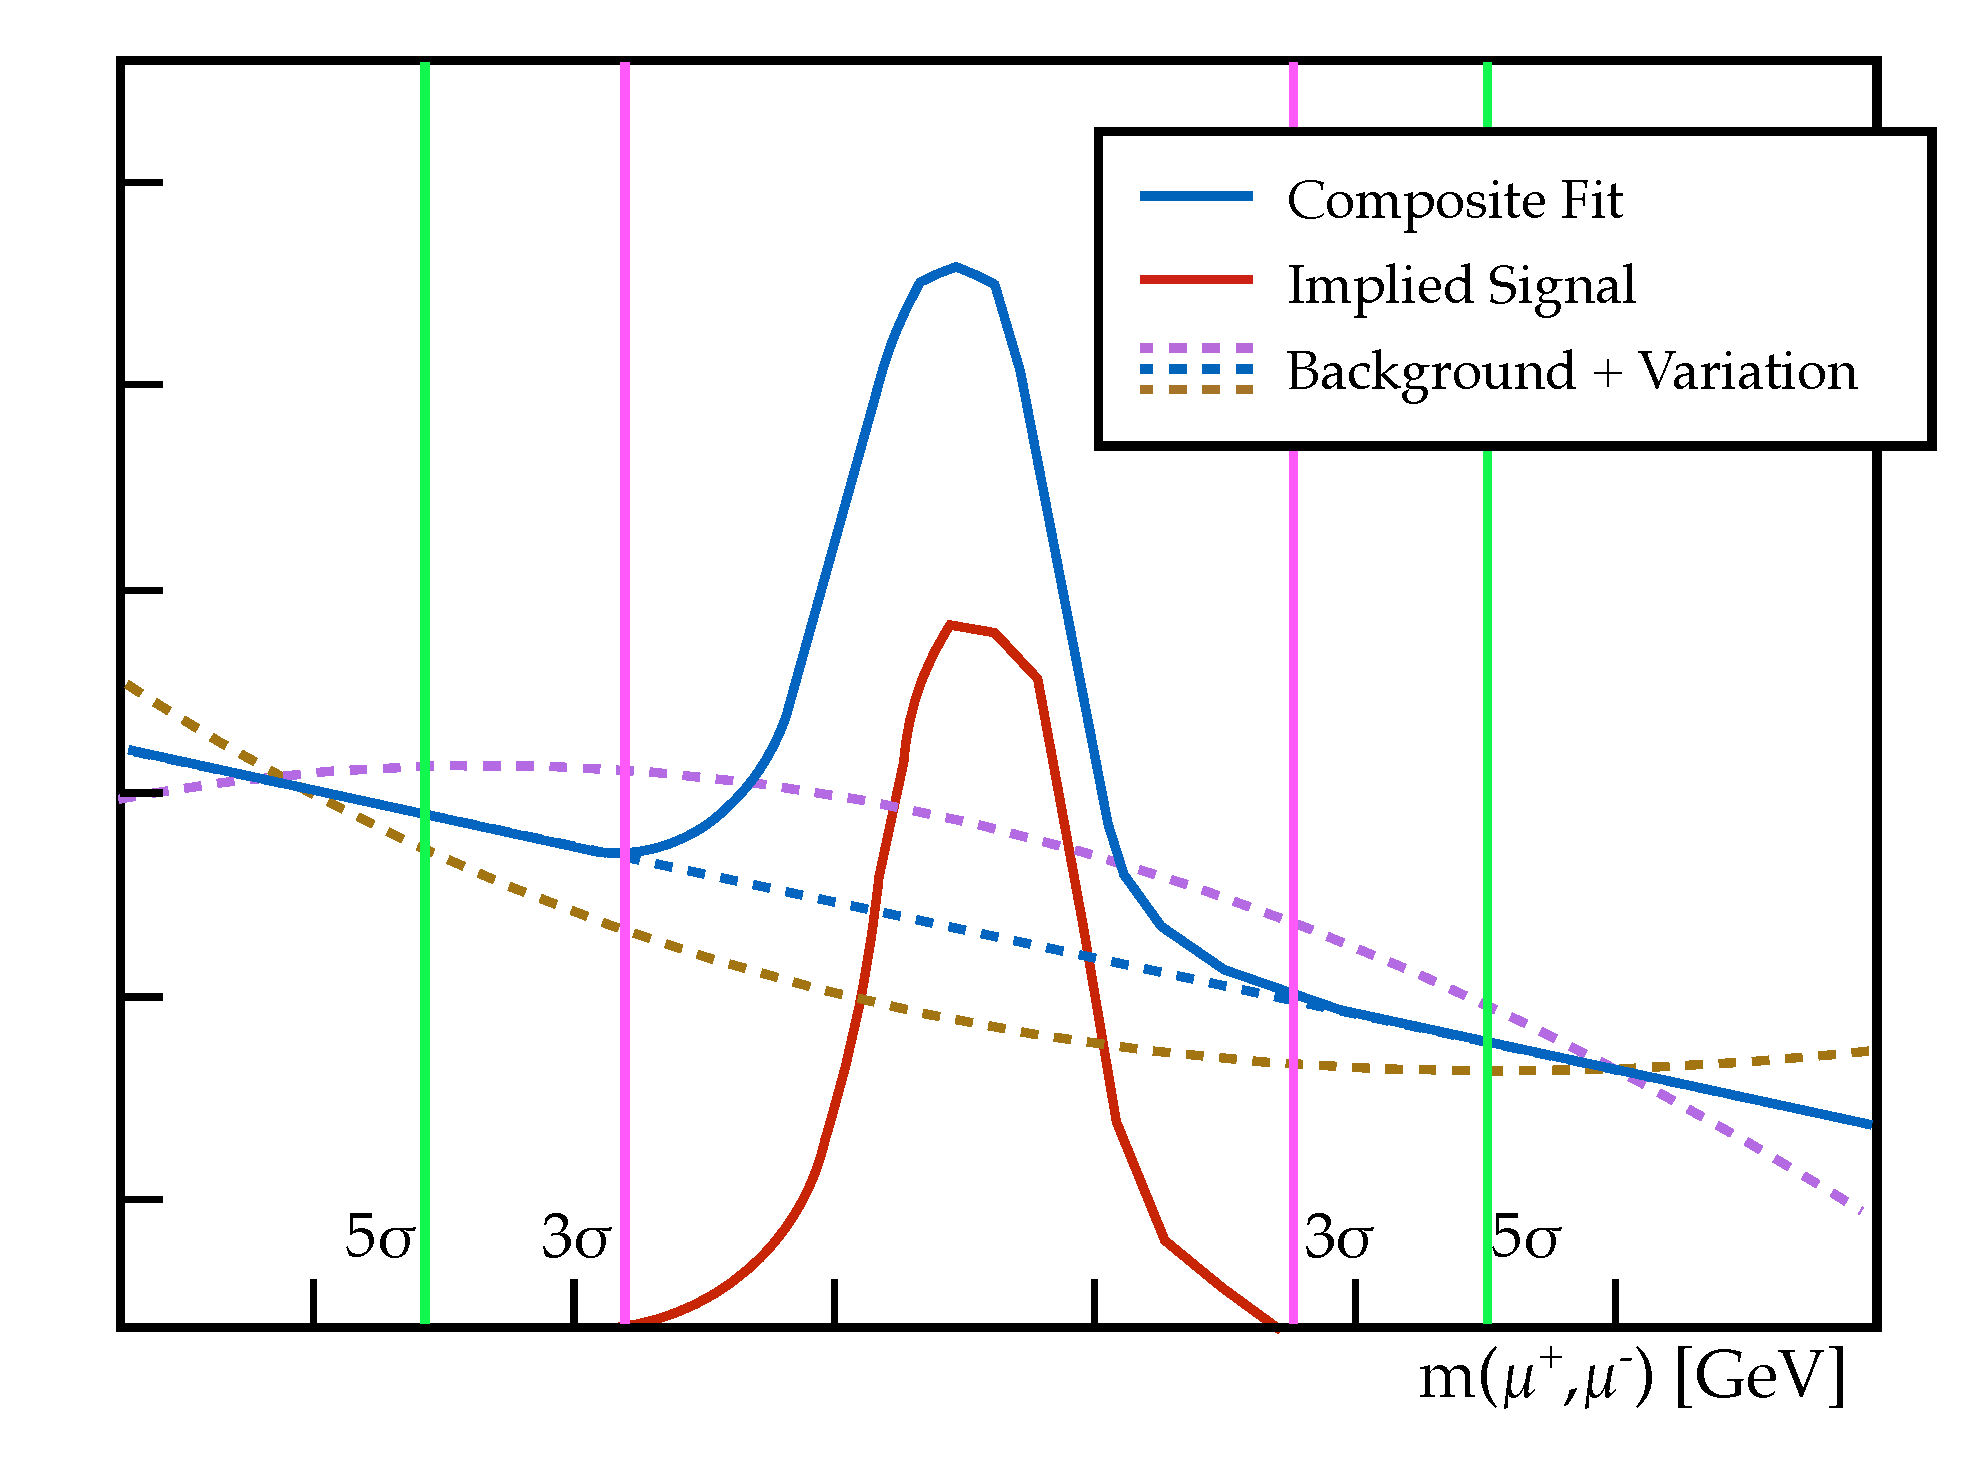
\includegraphics[width=0.85\textwidth]{PartCalibration2012/Plots/FittingExample.pdf}
  \caption{A diagram of the various components of the fit procedure. The composite fit is shown along with the corresponding implied signal and background. The two variations of the background shape are also shown.} \label{fig:CalibrationFittingExample}
\end{figure}

\subsection{Uncertainty Measurement}

The uncertainty on the efficiency is made of three components. First, the statistical uncertainty on the efficiency is estimated as a Binomial error:

\begin{equation}
  \delta\epsilon = \sqrt{\frac{\epsilon\times(1-\epsilon)}{N}}
\end{equation}

Where $\epsilon$ is the measured efficiency and N is, in this case the denominator of the efficiency measured.

Secondly, an uncertainty is associated with the fit to the background. This is done by taking the largest upward and downward fluctuations of the background by the uncertainty on the fit parameters of the background, and obtaining the maximum upward and downward effects on the efficiency. 
After the fit of the composite function is carried out, a downward variation of the background is defined as:

\begin{equation}
  f(x) = a_{\text{min}}x^{2} + b_{\text{max}}x + c_{\text{min}}\text{, where }p_{\text{max/min}}=p_{\text{central}}\pm\sigma_{p}
\end{equation}

Here the maximum and minimum of a parameter is obtained by varying the central value by the uncertainty obtained from the fit. The upward variation of the background fit is thus the opposite, defined as:

\begin{equation}
  f(x) = a_{\text{max}}x^{2} + b_{\text{min}}x + c_{\text{max}}
\end{equation}

These background variation then result in the maximum deviation from the nominal integral. Again Fig.~\ref{fig:CalibrationFittingExample} shows these two variations\footnote{The variation shown in the diagram is very exagerated and meant for illustration purposes}. The uncertainty on the efficiency is then determined by obtaining the maximum efficiency in both directions. If the nominal efficiency is defined as:

\begin{equation}
  \epsilon_{\text{nominal}} = \frac{N_{numerator}}{N_{denominator}}
\end{equation}

Then the variations are defined as follows:

\begin{equation}
  \epsilon_{\text{up}} = \frac{N^{down}_{numerator}}{N^{nominal}_{denominator}}\text{, }\,
  \epsilon_{\text{down}} = \frac{N^{nominal}_{numerator}}{N^{up}_{denominator}}
\end{equation}

Finally the uncertainty on the background is given by adding the differences between $\epsilon{\text{up}}$ and $\epsilon{\text{down}}$ and the nominal efficiency, in quadrature:

\begin{equation}
  \sigma_{\text{bkg}} = \sqrt{|\epsilon_{\text{up}}-\epsilon|^{2}+|\epsilon_{\text{down}}-\epsilon|^{2}}
\end{equation}

The final component of the uncertainty is constructed by varying the integration window. The nominal value is defined as $3\sigma$ away from the center of the fitted gaussian, where again $\sigma$ is the FWHM of the same fitted gaussian. An uncertainty is constructed by measuring the efficiency with a wide integration window corresponding to $5\sigma$. The integration window uncertainty is defined as:

\begin{equation}
  \sigma_{\text{window}} = |\epsilon_{5\sigma}-\epsilon_{3\sigma}|
\end{equation}

Finally, the total uncertainty on the efficiency is given by the sum in quadrature of the all uncertainty components. The uncertainty on the efficiency is then carried over to the scale factor determination.

An example of the fitting procedure applied is shown in Fig.~\ref{fig:CalibrationFittingResult} for both tag and probes at probe level and at muon probe level. Note that as expected the muon probe contains far less background.

\begin{figure}[thbp]
  \centering
  \begin{subfigure}[b]{0.85\textwidth}
  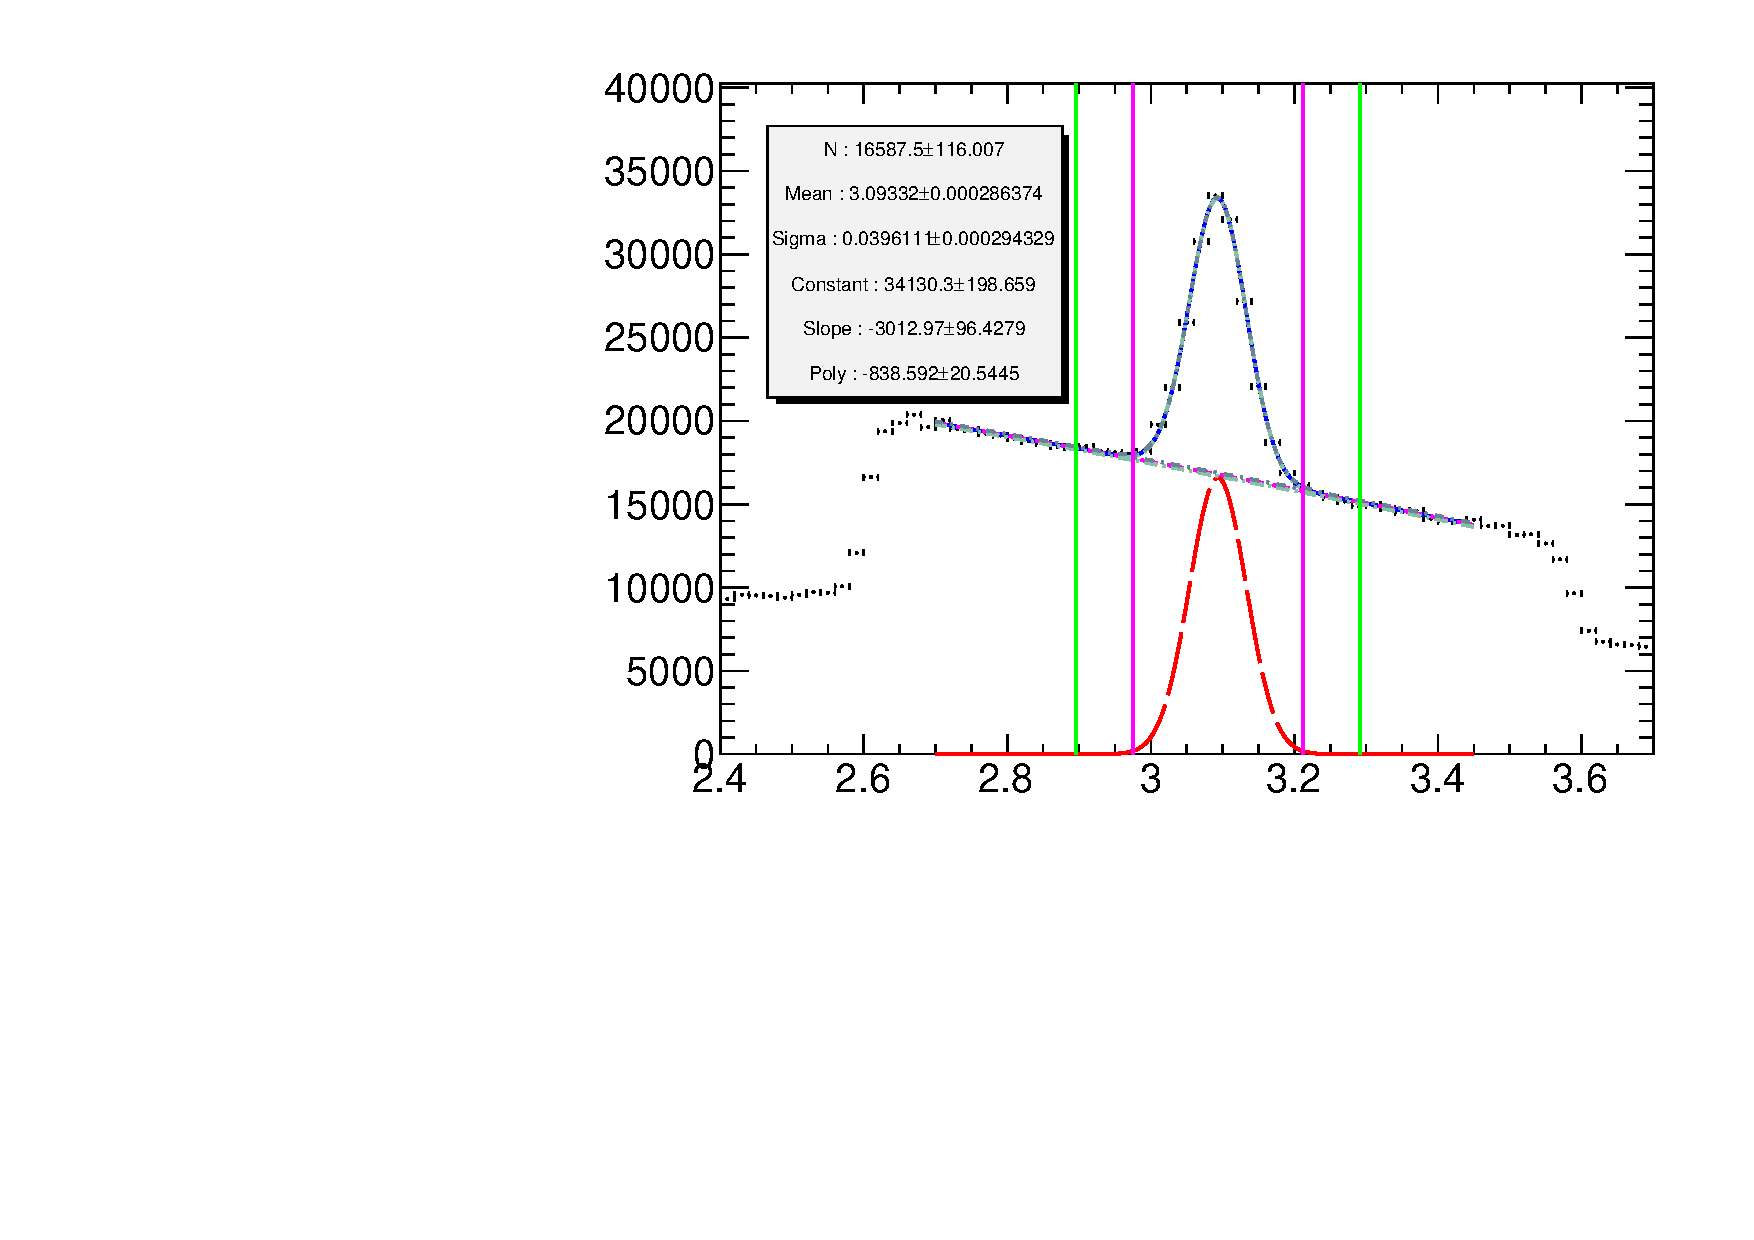
\includegraphics[width=\textwidth]{PartCalibration2012/Plots/Kinematics/Data_InvMass_pt_5_6_barrel_probe.pdf}
    \caption{Probe level}
  \end{subfigure}

  \begin{subfigure}[b]{0.85\textwidth}
    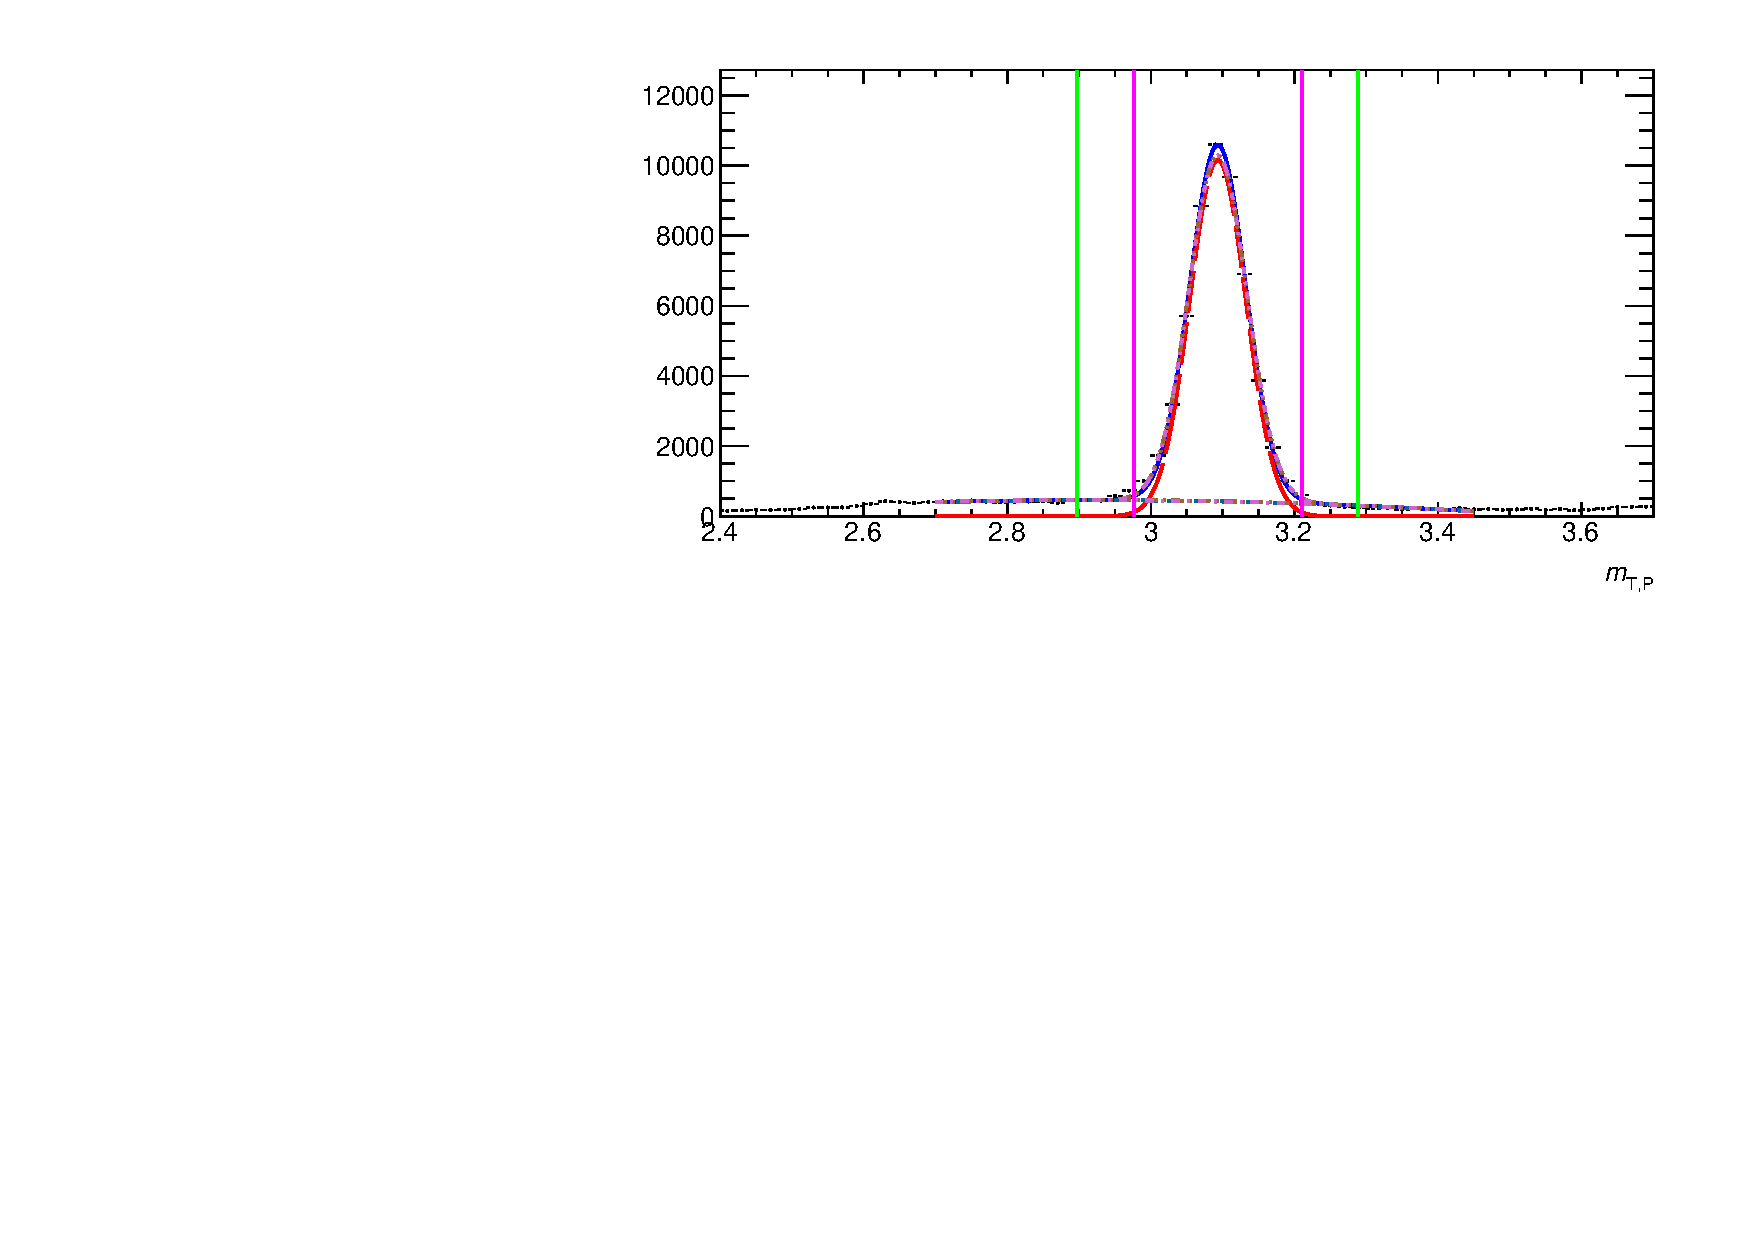
\includegraphics[width=\textwidth]{PartCalibration2012/Plots/Kinematics/Data_InvMass_pt_5_6_barrel_muonprobe.pdf}
    \caption{Muon probe level}   
  \end{subfigure} 
  \caption{Invariant mass distributions of tag and probe pairs at a) probe level and at b) muon probe level in collision data. Note the various components of the fit as well as the variations on the background fits and the $3\sigma$ and $5\sigma$ integration windows used for systematics. Note the fit parameters and their respective uncertainties} \label{fig:CalibrationFittingResult}
\end{figure}

\section{Efficiencies} \label{sec:CalibrationEfficiencies}

The efficiency is monitored as a function of a variety of kinematic variables, including isolation variables, transverse momentum and angular position of the probe.

\subsection{Isolation dependence} \label{sec:CalibrationEfficienciesIsolation}

The muons from \jpsi\ used in this calibration are produced in isolation, there is very little energetic activity surrounding them in the detector. In contrast muons from semileptonic decay of $b$-quarks in \ttbar\ events are produced amongst the numerous components of the $b$-jets. Thus it is important to ensure that the performance of the \xsm\ tagger is not affected by the isolation of the muon for a calibration on \jpsi\ events to be applicable. In this calibration as, in the 2011 analysis nine isolation variables are considered. The so-called etcone20, 30 and 40 correspond to the transverse energy surrounding the muon in a cone of size $\Delta R=0.2,0.3,0.4$ respectively. Additionally ptcone20, 30 and 40 and nucone20, 30, 40 correspond to the sum of transverse momentum and the number of tracks surrounding the muon, respectively. All nine isolation variables exclude the muon itself in a cone of size 0.1 and include various corrections for known energy losses, momentum leakages between adjacent clusters in the detector and the effects of pile-up.

As in the 2011 analysis there appears to be no dependence of the scale factor on any of the isolation variables examined as can be seen from Fig.~\ref{fig:Calibration2011Iso}.

\begin{figure}[phtb]
  \centering
    % Subfigure ETCone20
    \begin{subfigure}[b]{0.31\textwidth}
      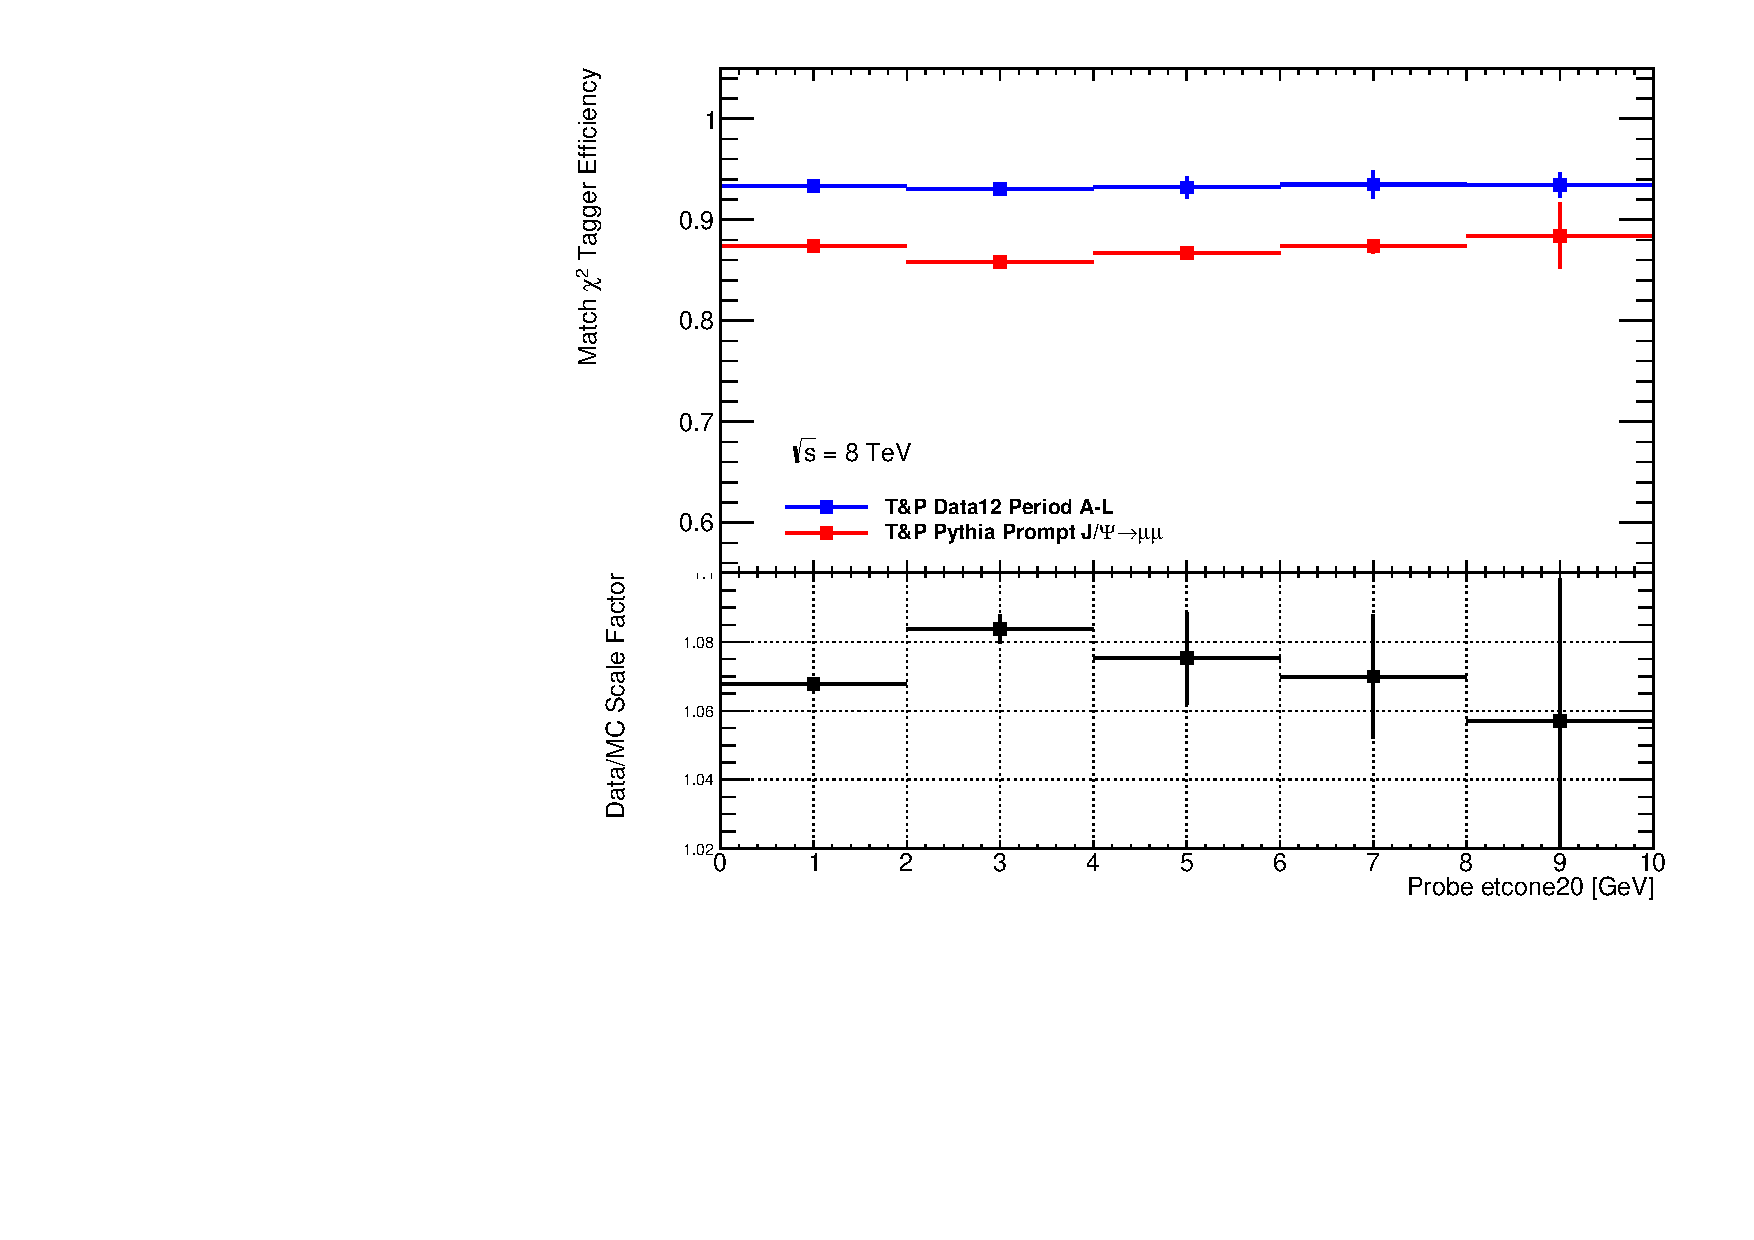
\includegraphics[width=\textwidth]{PartCalibration2012/Plots/SFPlots/etcone20_smt.pdf}
      \caption{$\sum E_{T}$ in cone $\Delta R=0.2$} \label{fig:Alleffsfetcone20}
    \end{subfigure}
    ~
    % Subfigure ETCone30
    \begin{subfigure}[b]{0.31\textwidth}
      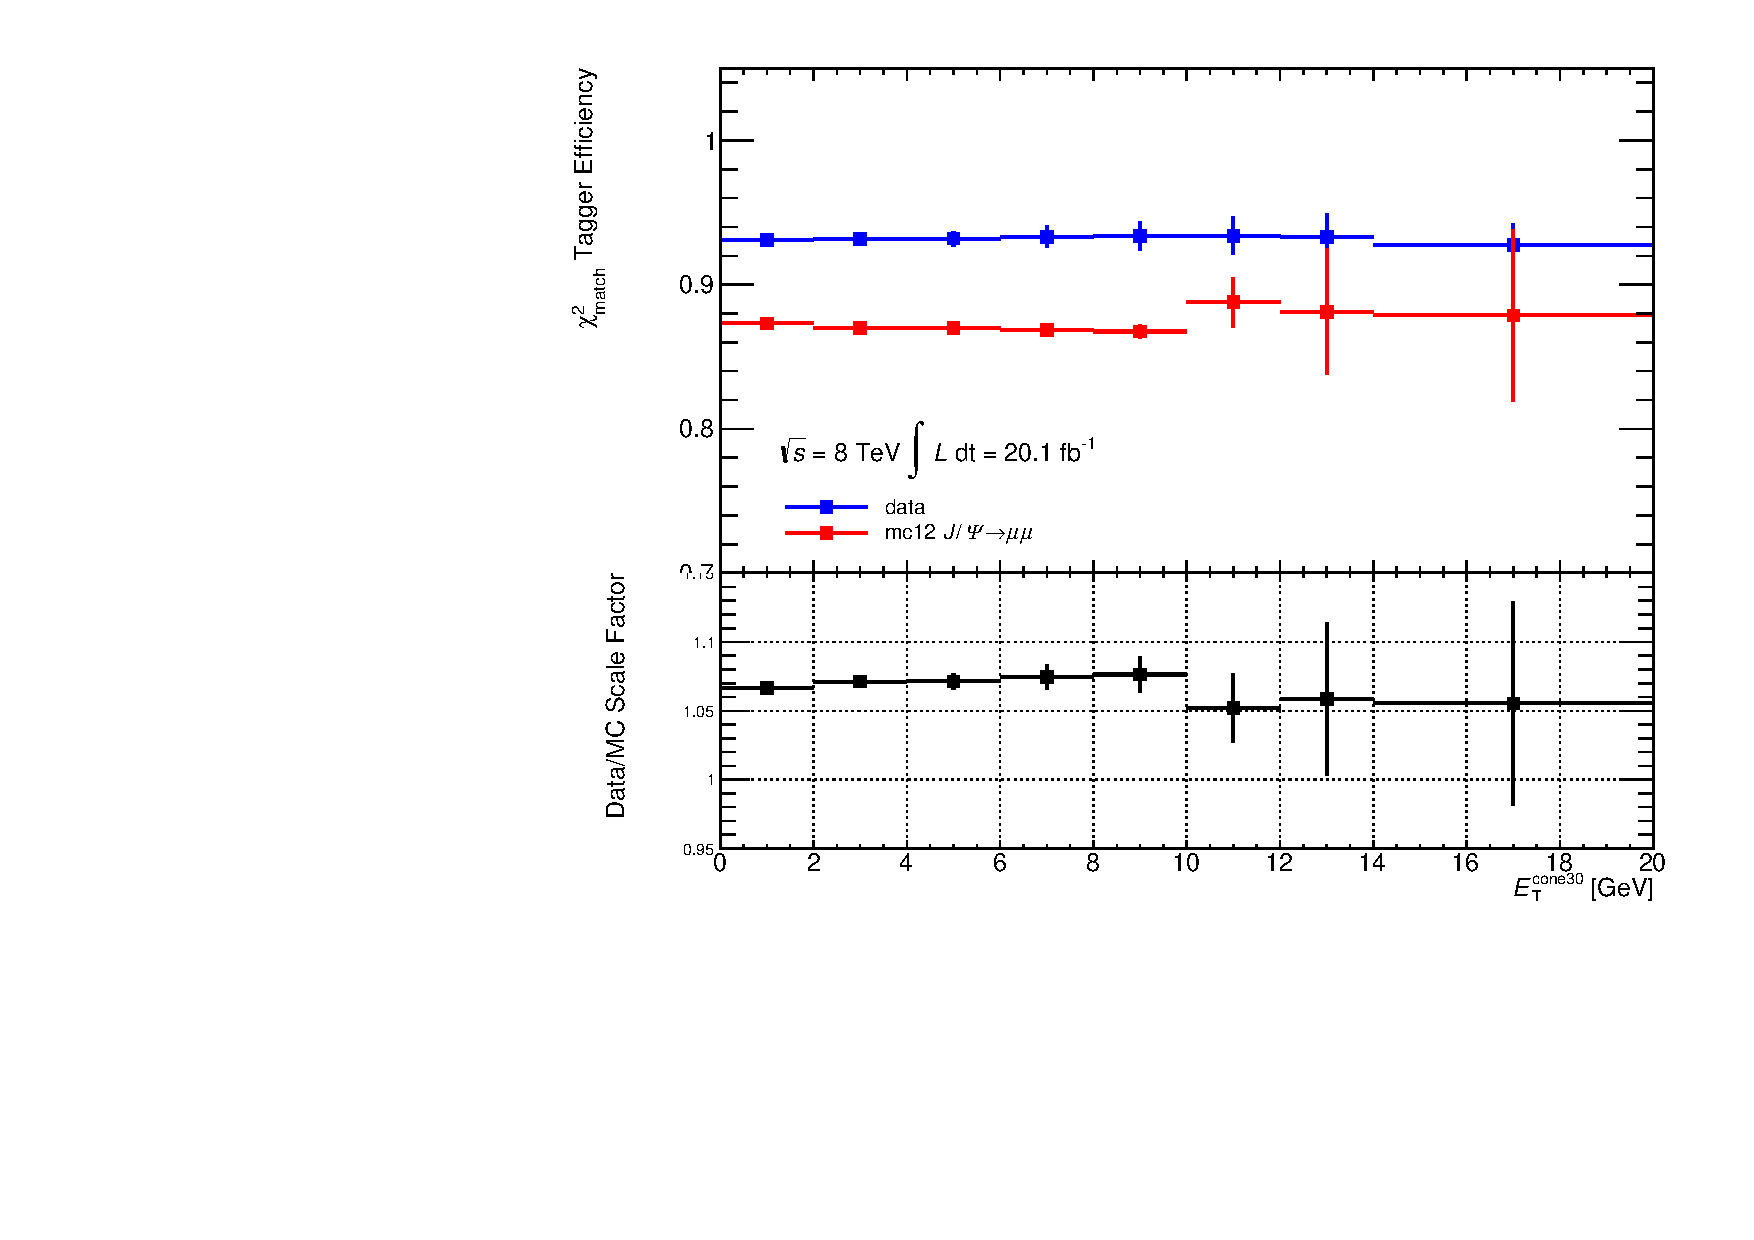
\includegraphics[width=\textwidth]{PartCalibration2012/Plots/SFPlots/etcone30_smt.pdf}
      \caption{$\sum E_{T}$ in cone $\Delta R=0.3$} \label{fig:Alleffsfetcone30}
    \end{subfigure}
    ~
    % Subfigure ETCone40
    \begin{subfigure}[b]{0.31\textwidth}
      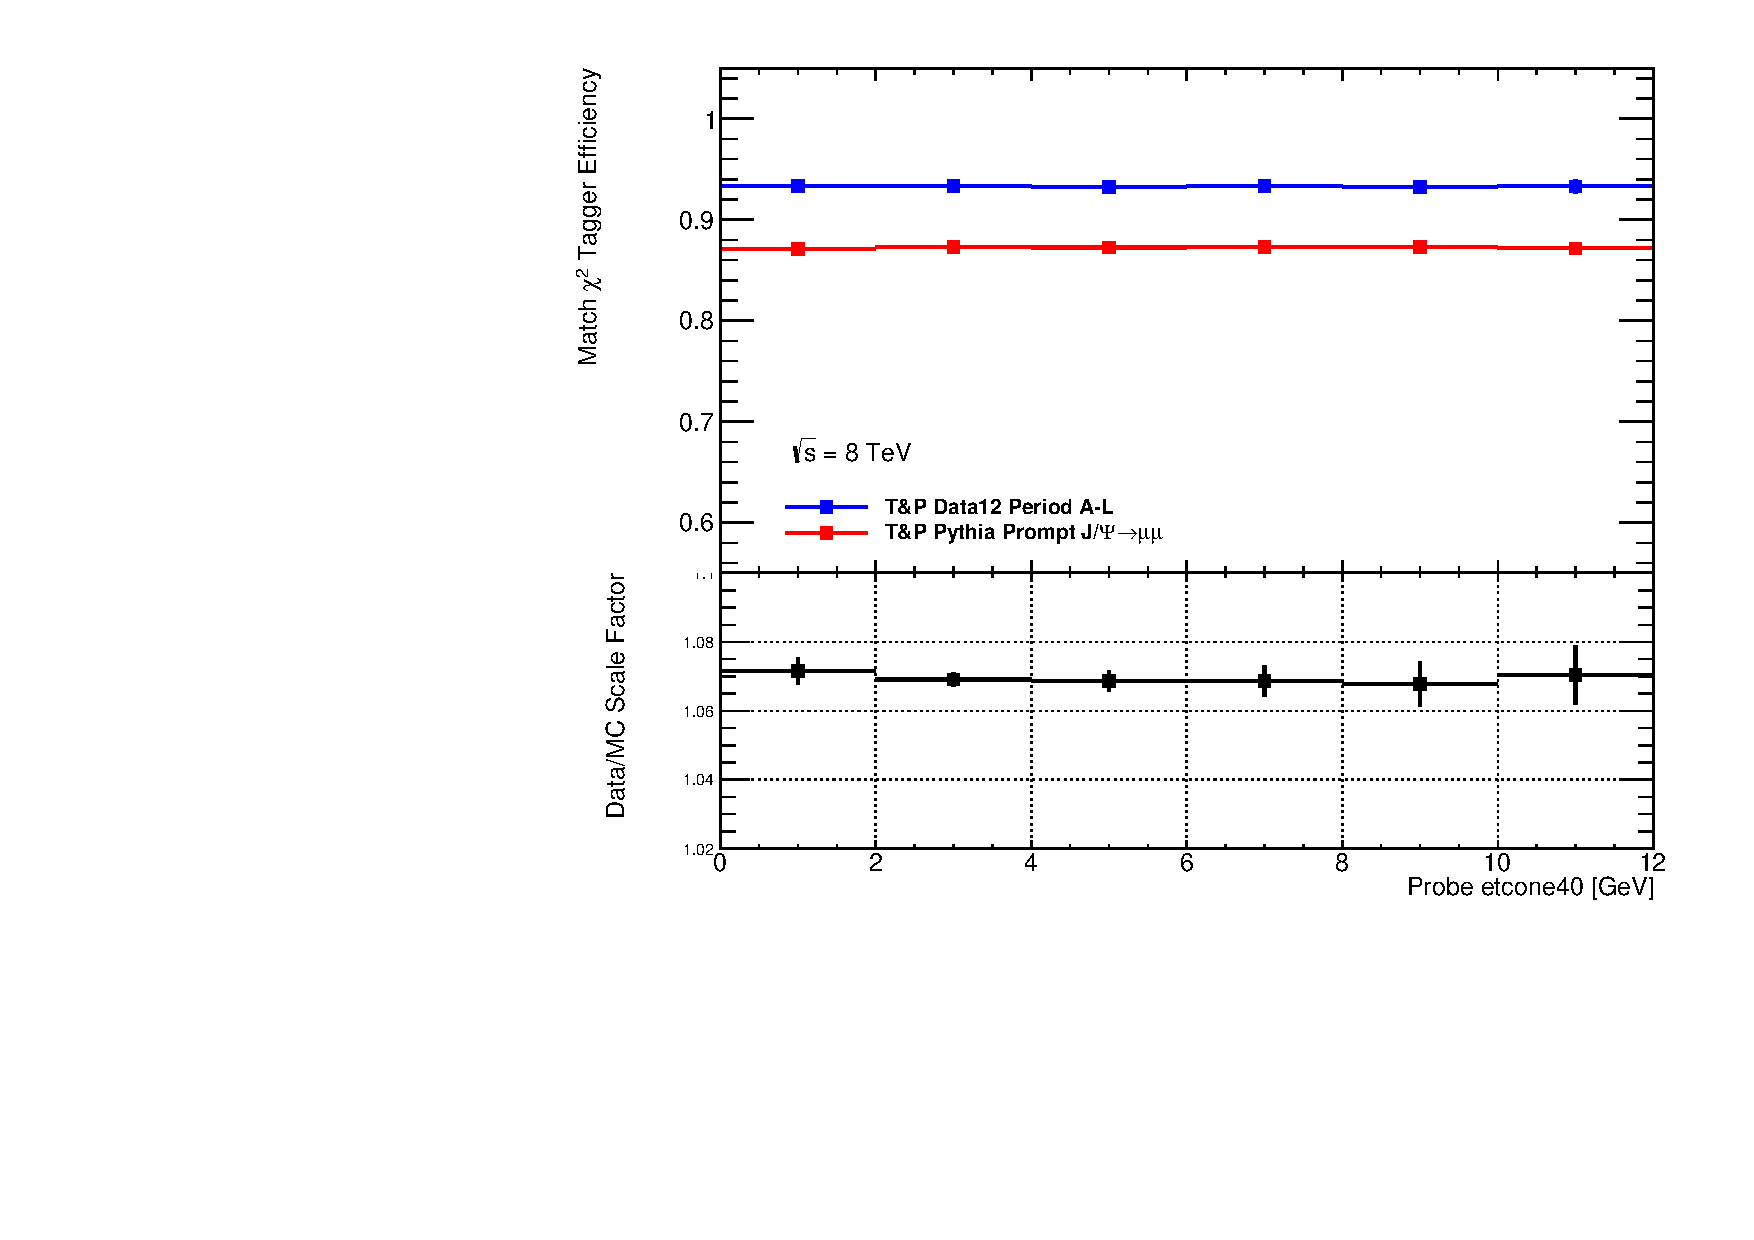
\includegraphics[width=\textwidth]{PartCalibration2012/Plots/SFPlots/etcone40_smt.pdf}
      \caption{$\sum E_{T}$ in cone $\Delta R=0.4$}\label{fig:Alleffsfetcone40}
    \end{subfigure}
    ~
    % ptcone20
    \begin{subfigure}[b]{0.31\textwidth}
      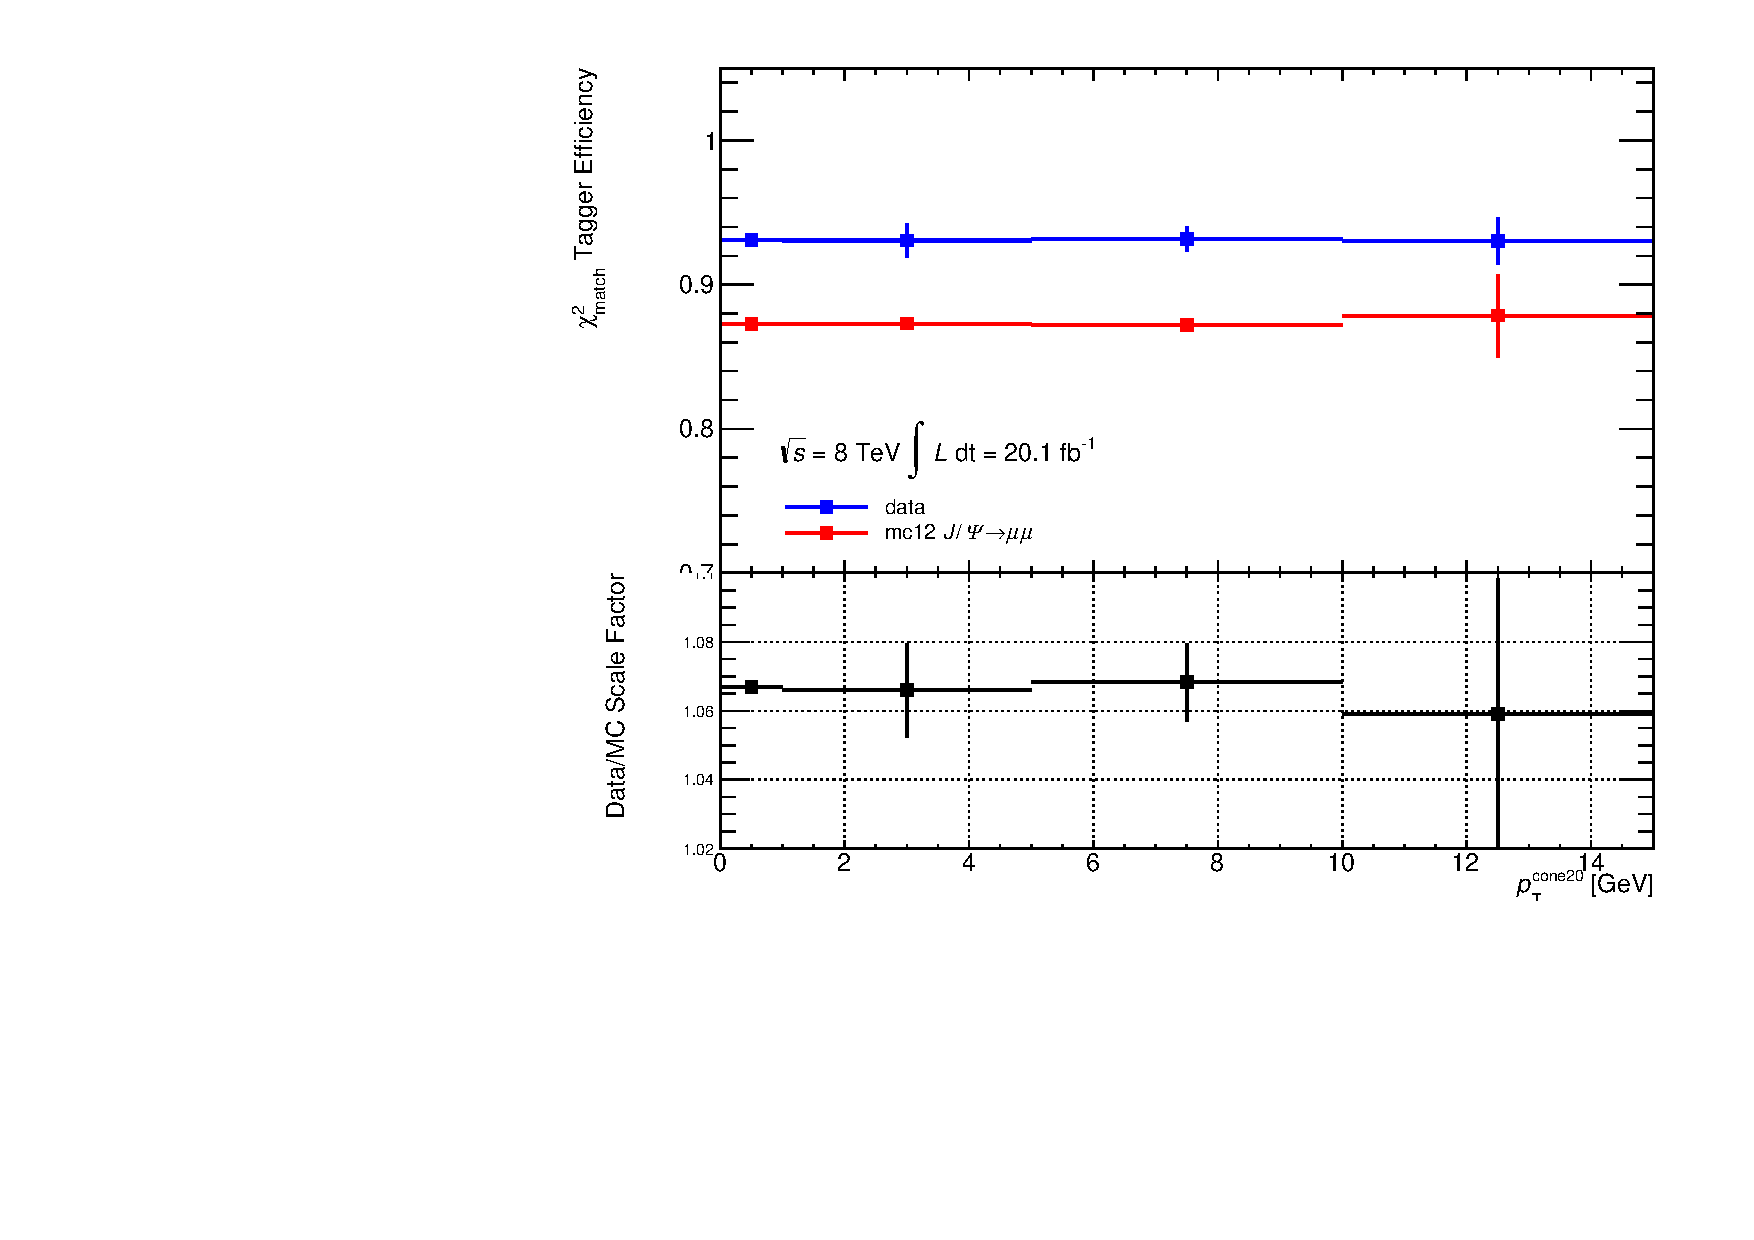
\includegraphics[width=\textwidth]{PartCalibration2012/Plots/SFPlots/ptcone20_smt.pdf}
      \caption{$\sum p_{T}$ in cone $\Delta R=0.2$} \label{fig:Alleffsfptcone20}
    \end{subfigure}
    ~
    %ptcone30
    \begin{subfigure}[b]{0.31\textwidth}
      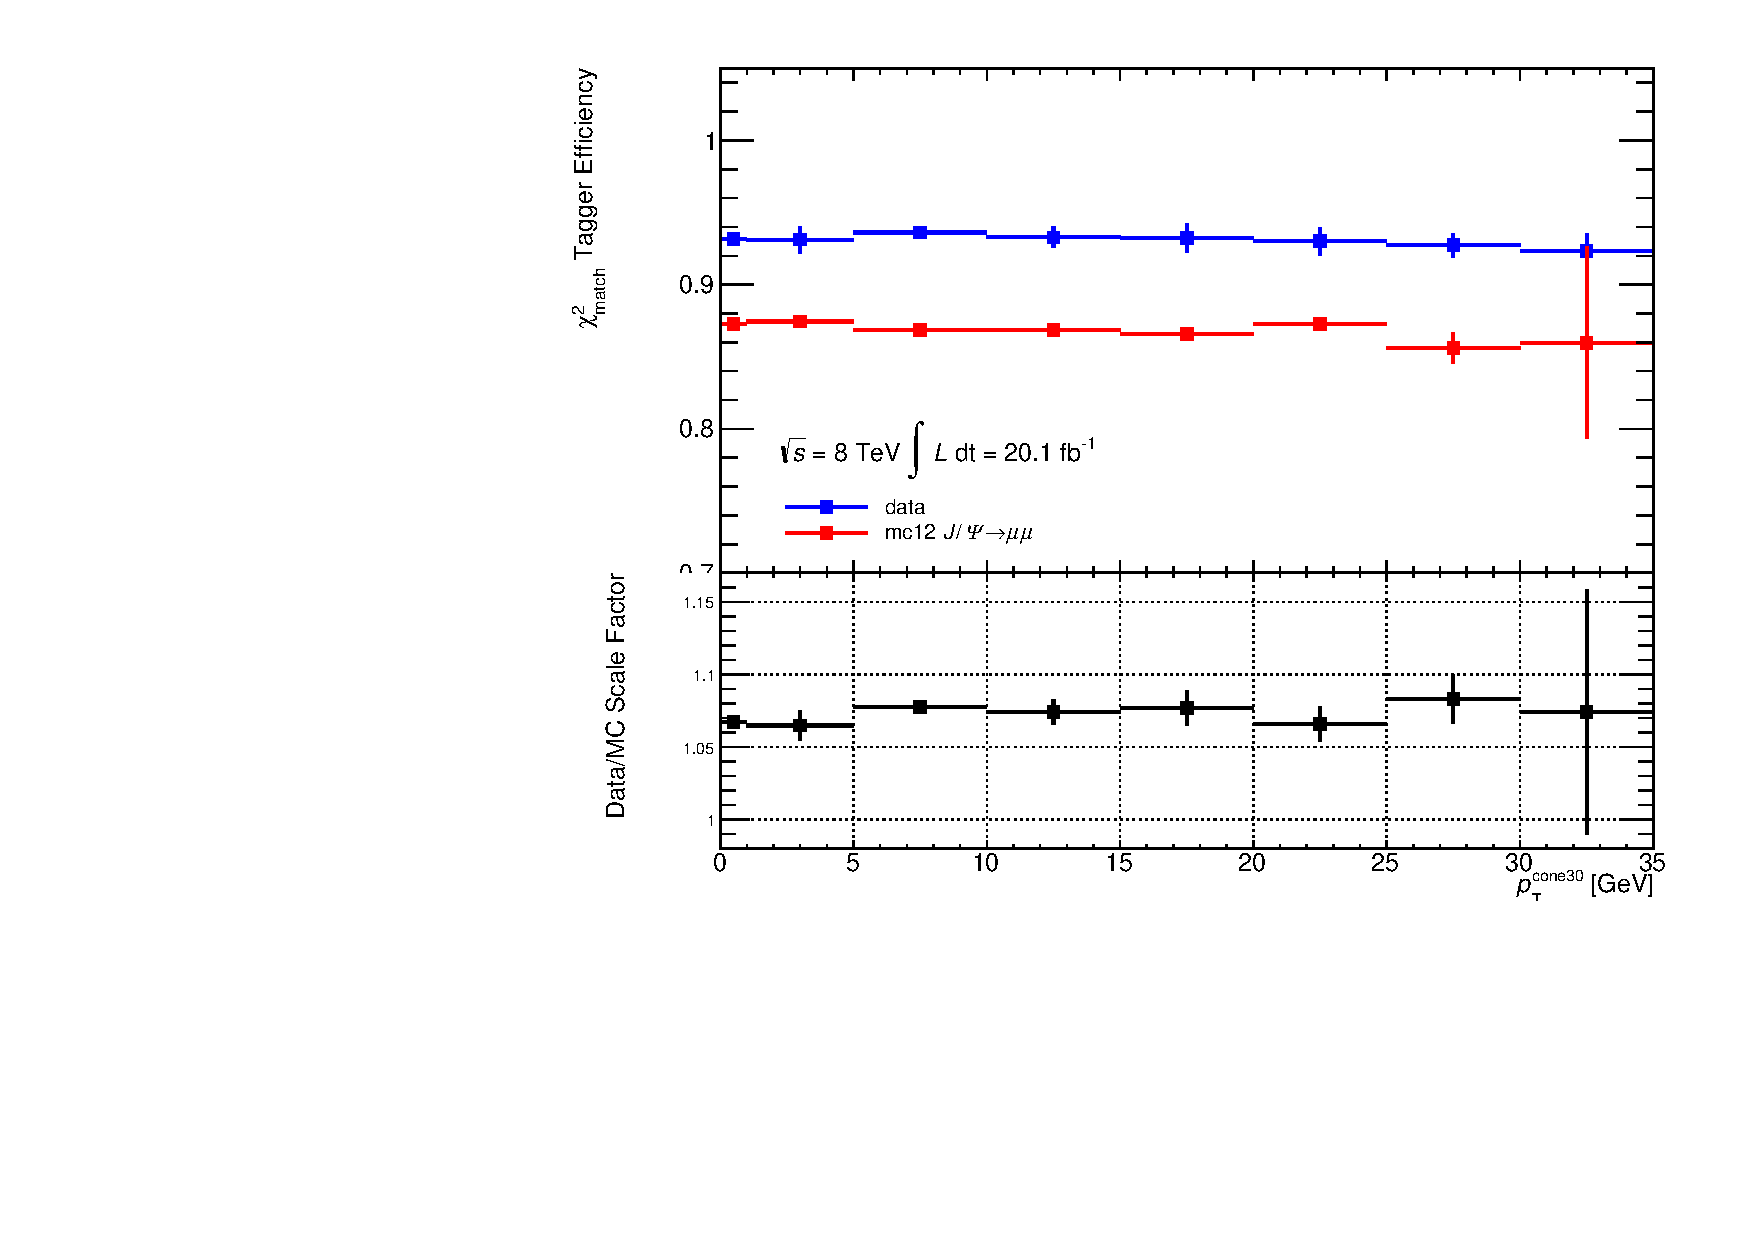
\includegraphics[width=\textwidth]{PartCalibration2012/Plots/SFPlots/ptcone30_smt.pdf}
      \caption{$\sum p_{T}$ in cone $\Delta R=0.3$} \label{fig:Alleffsfptcone30}
    \end{subfigure}
    ~
    % ptcone40
    \begin{subfigure}[b]{0.31\textwidth}
      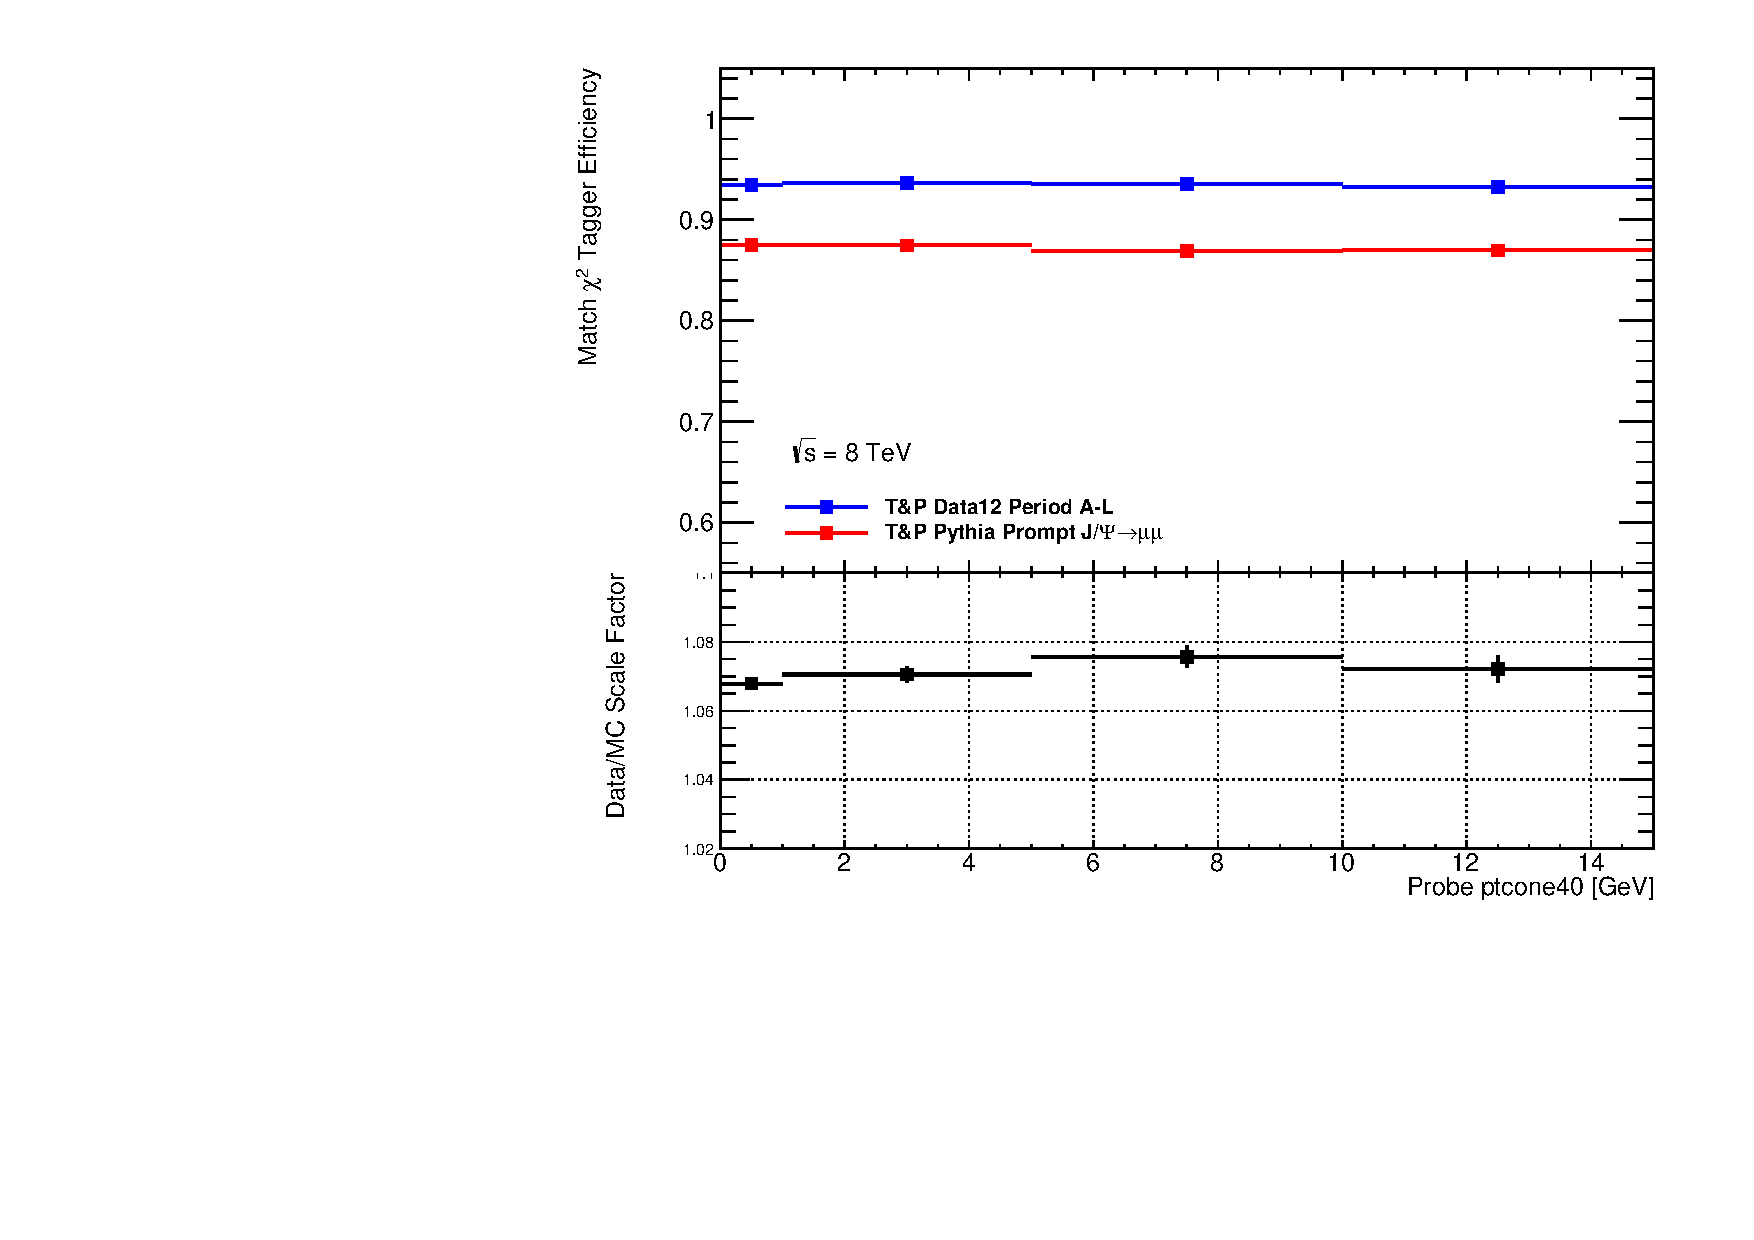
\includegraphics[width=\textwidth]{PartCalibration2012/Plots/SFPlots/ptcone40_smt.pdf}
      \caption{$\sum p_{T}$ in cone $\Delta R=0.4$} \label{fig:Alleffsfptcone40}
    \end{subfigure}
    ~
    % nucone20
    \begin{subfigure}[b]{0.31\textwidth}
      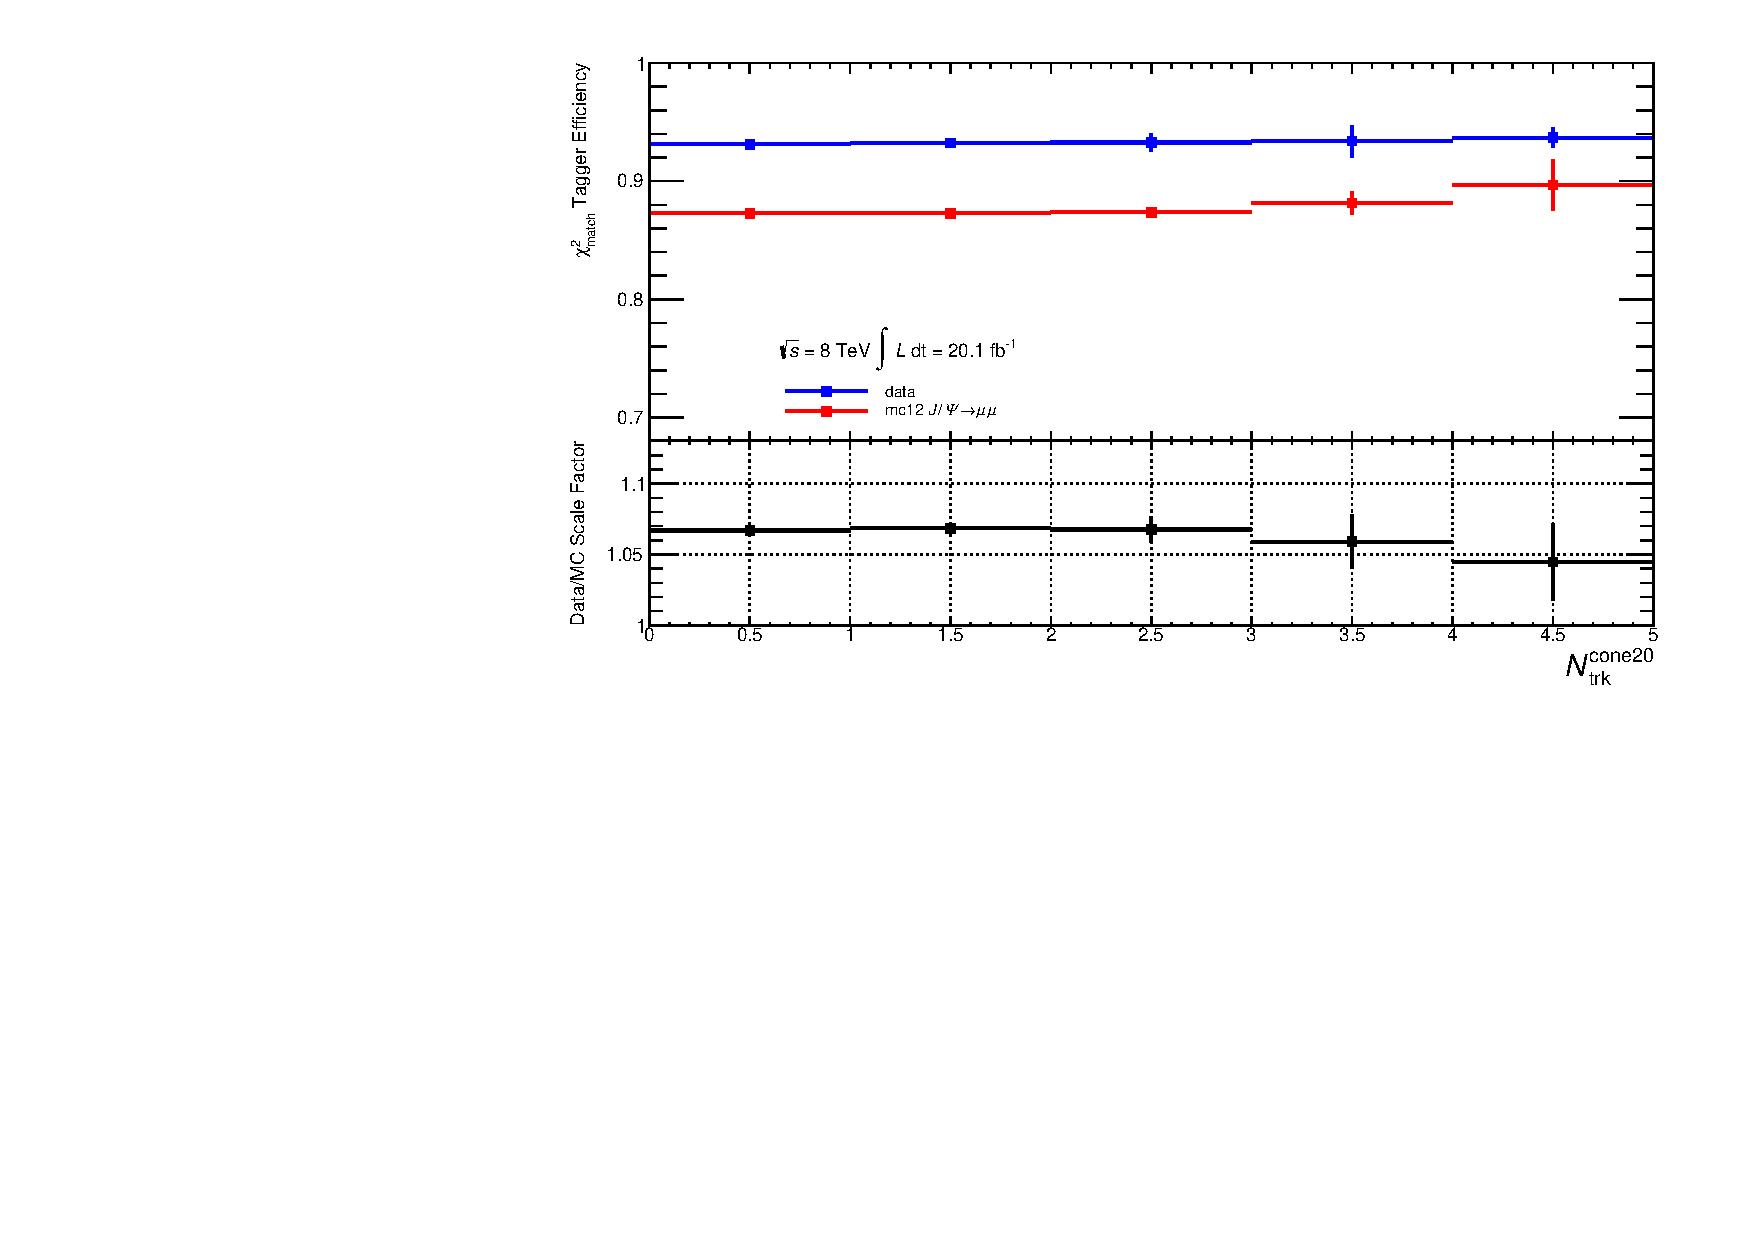
\includegraphics[width=\textwidth]{PartCalibration2012/Plots/SFPlots/nucone20_smt.pdf}  
      \caption{$N_{\textrm{trk}}$ in cone $\Delta R=0.2$} \label{fig:Alleffsfnucone20}
    \end{subfigure}
    ~
    % nucone30
    \begin{subfigure}[b]{0.31\textwidth}
      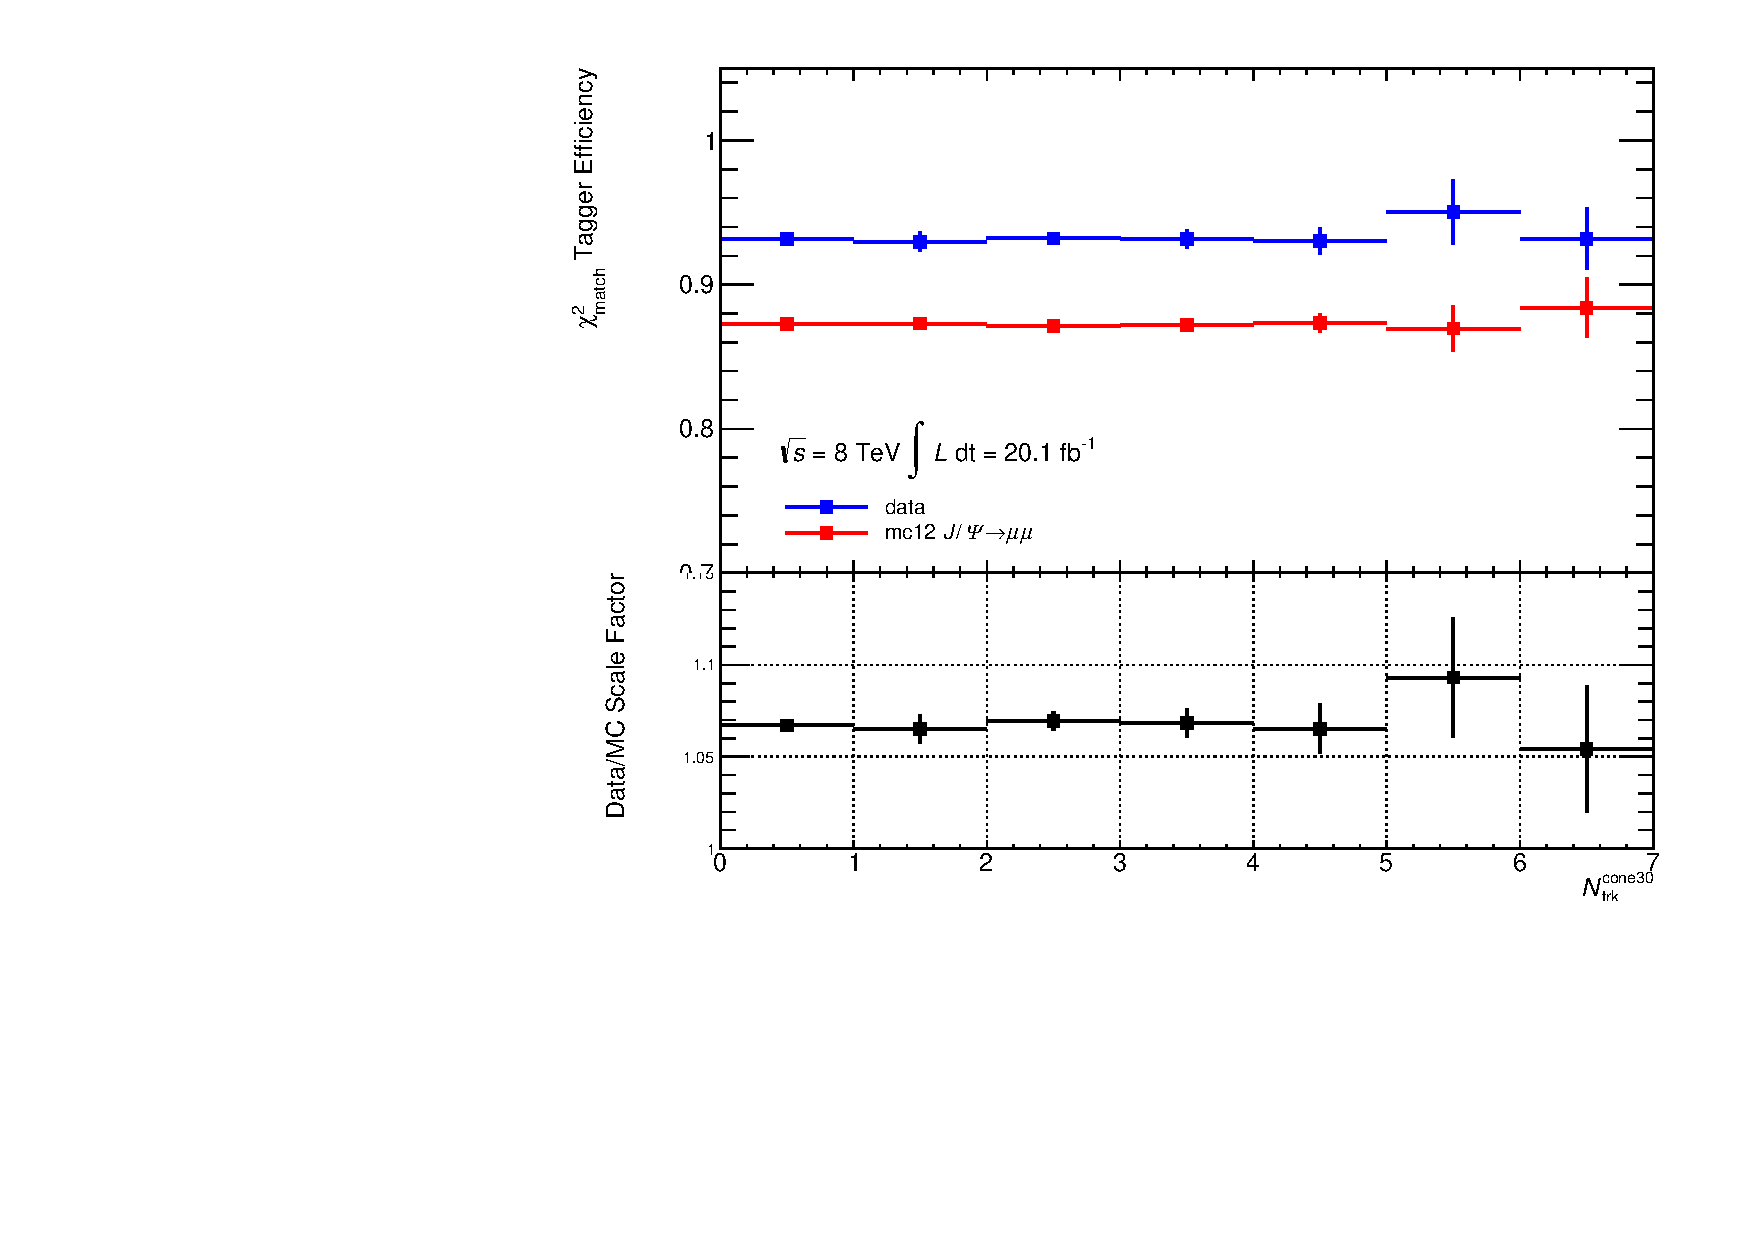
\includegraphics[width=\textwidth]{PartCalibration2012/Plots/SFPlots/nucone30_smt.pdf}
      \caption{$N_{\textrm{trk}}$ in cone $\Delta R=0.3$} \label{fig:Alleffsfnucone30}
    \end{subfigure}
    ~
    % nucone40
    \begin{subfigure}[b]{0.31\textwidth}
      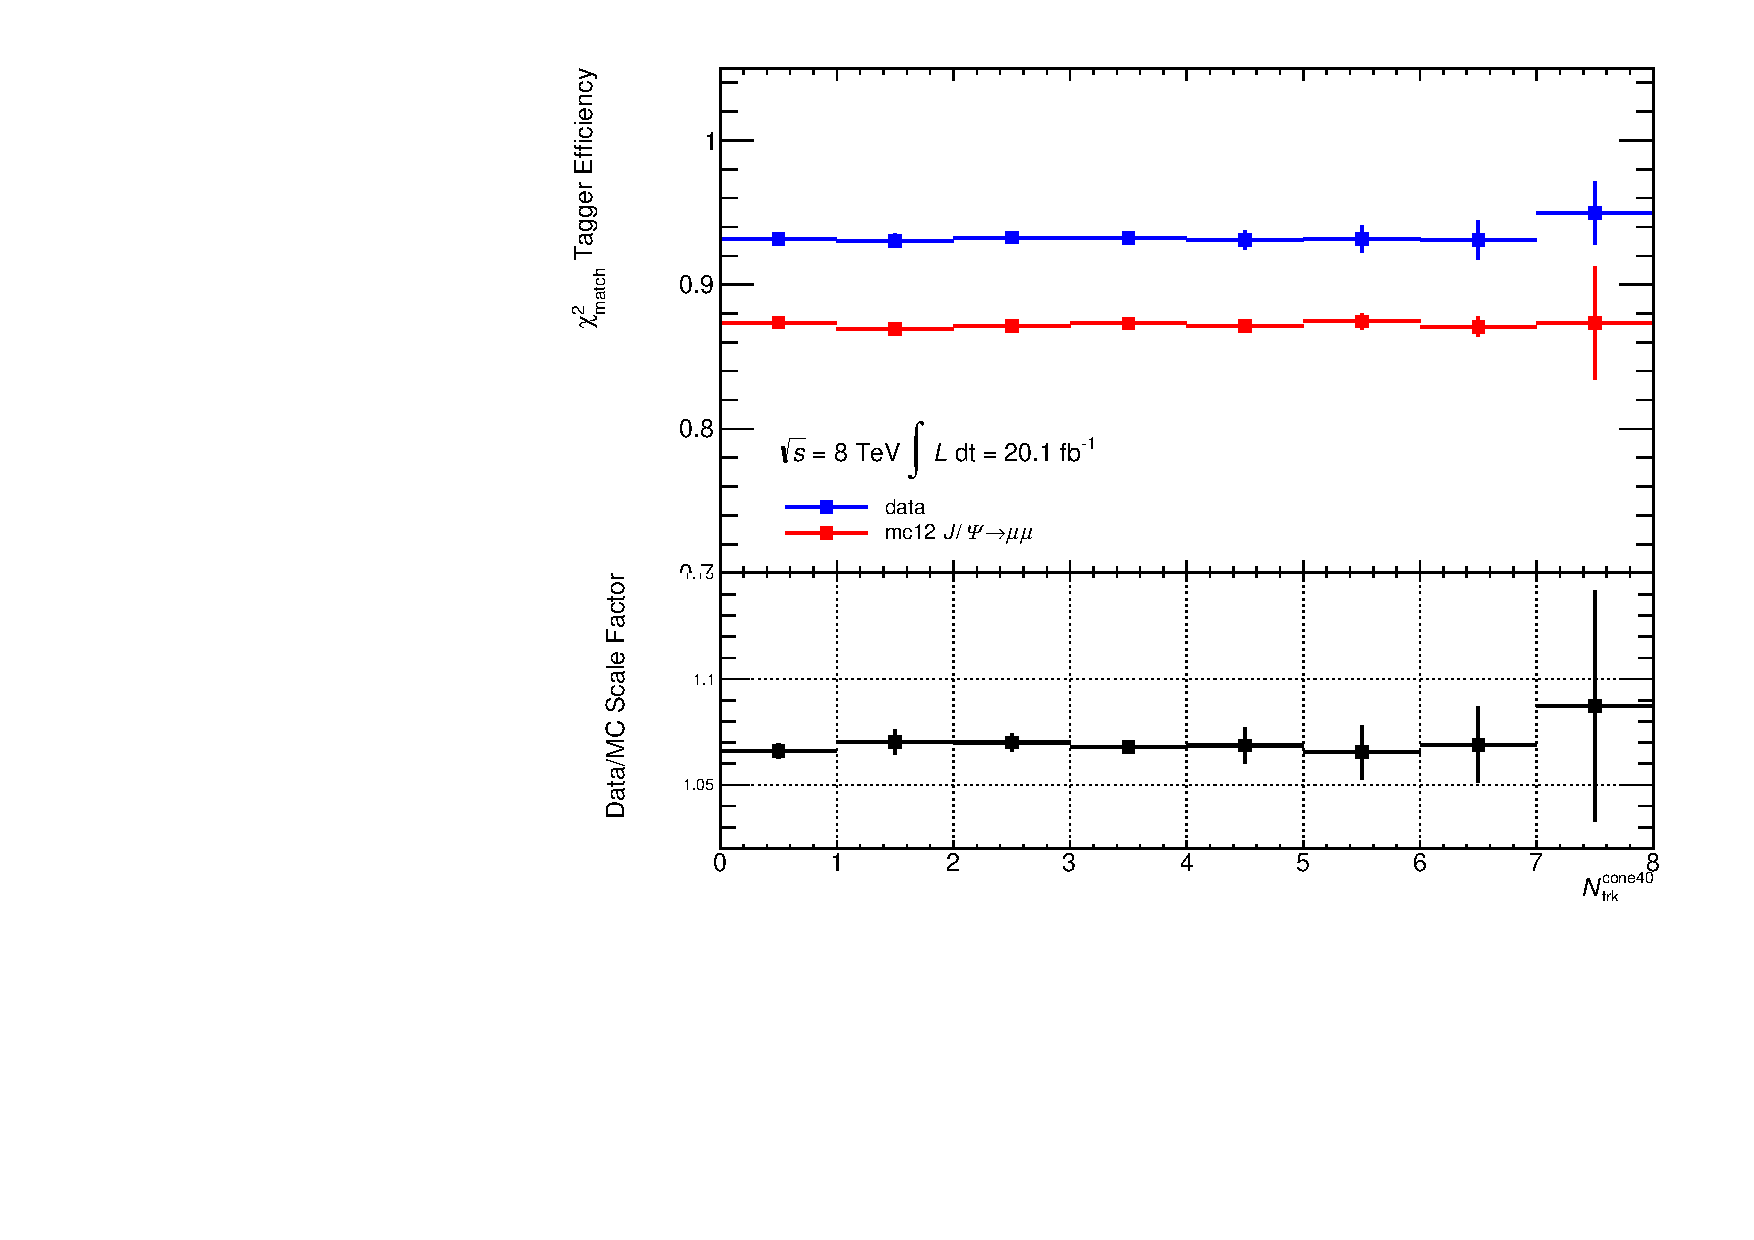
\includegraphics[width=\textwidth]{PartCalibration2012/Plots/SFPlots/nucone40_smt.pdf}
      \caption{$N_{\textrm{trk}}$ in cone $\Delta R=0.4$} \label{fig:Alleffsfnucone40}
    \end{subfigure}
  \caption{\xsd\ efficiencies and scale factor with respect various isolation variables.} \label{fig:Calibration2011Iso}
\end{figure}

The dependence on each isolation variable is measured in a range dictated by the available statistics. Given the isolated nature of muons in \jpsi\ events limits the number of muons available at higher pt/et/nucone values.

\subsection{2011 Calibration}

% talk about the results from 2011

\subsection{Efficiency Binning}

The efficiencies are measured across the $|\eta|$ range of the ATLAS detector in regions defined in Table~\ref{tab:CalibrationEtaRegions}. As in 2011, the efficiency is expected to be depedent on the region of the detector where the muon probe emerges.

\begin{table}[thbp]
  \centering
  \caption{Pseudorapidity regions of the ATLAS detector} \label{tab:CalibrationEtaRegions}
  \begin{tabular}{|c|c|}
    \hline 
    $|\eta|$ range & Name \\ \hline \hline
    $0.0<|\eta|<0.1$ & Crack \\
    $0.1<|\eta|<1.1$ & Barrel \\
    $1.1<|\eta|<1.3$ & Transition \\
    $1.3<|\eta|<2.0$ & Endcap \\
    $2.0<|\eta|<2.5$ & Forward \\
    \hline
  \end{tabular}
\end{table}

\begin{figure}[tbhp]
  \centering
  \begin{subfigure}[b]{0.85\textwidth}
    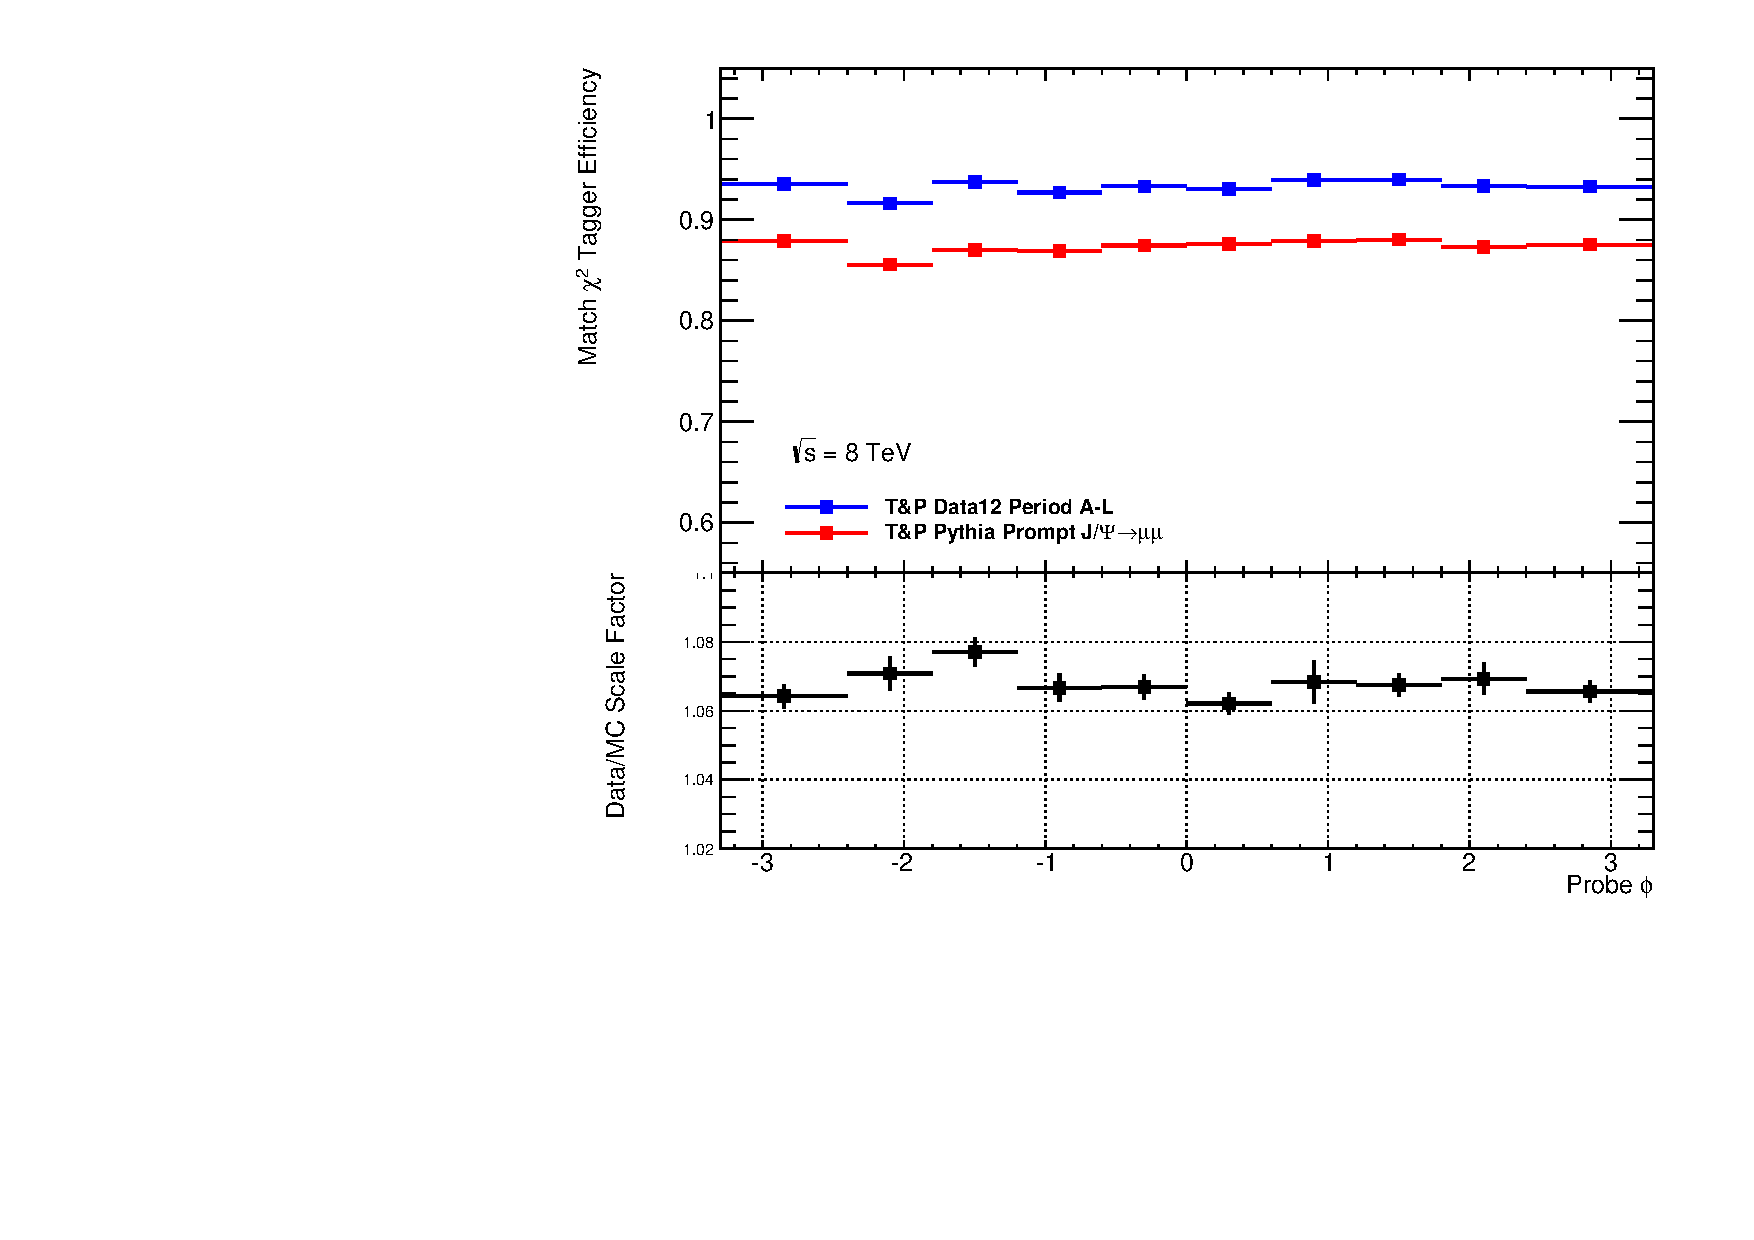
\includegraphics[width=\textwidth]{PartCalibration2012/Plots/SFPlots/phi_smt.pdf}
    \caption{\xsm\ efficiency and scale factor as a function $\phi$ of the probe muon} \label{fig:CalibrationPhi}
  \end{subfigure}

  \begin{subfigure}[b]{0.85\textwidth}
    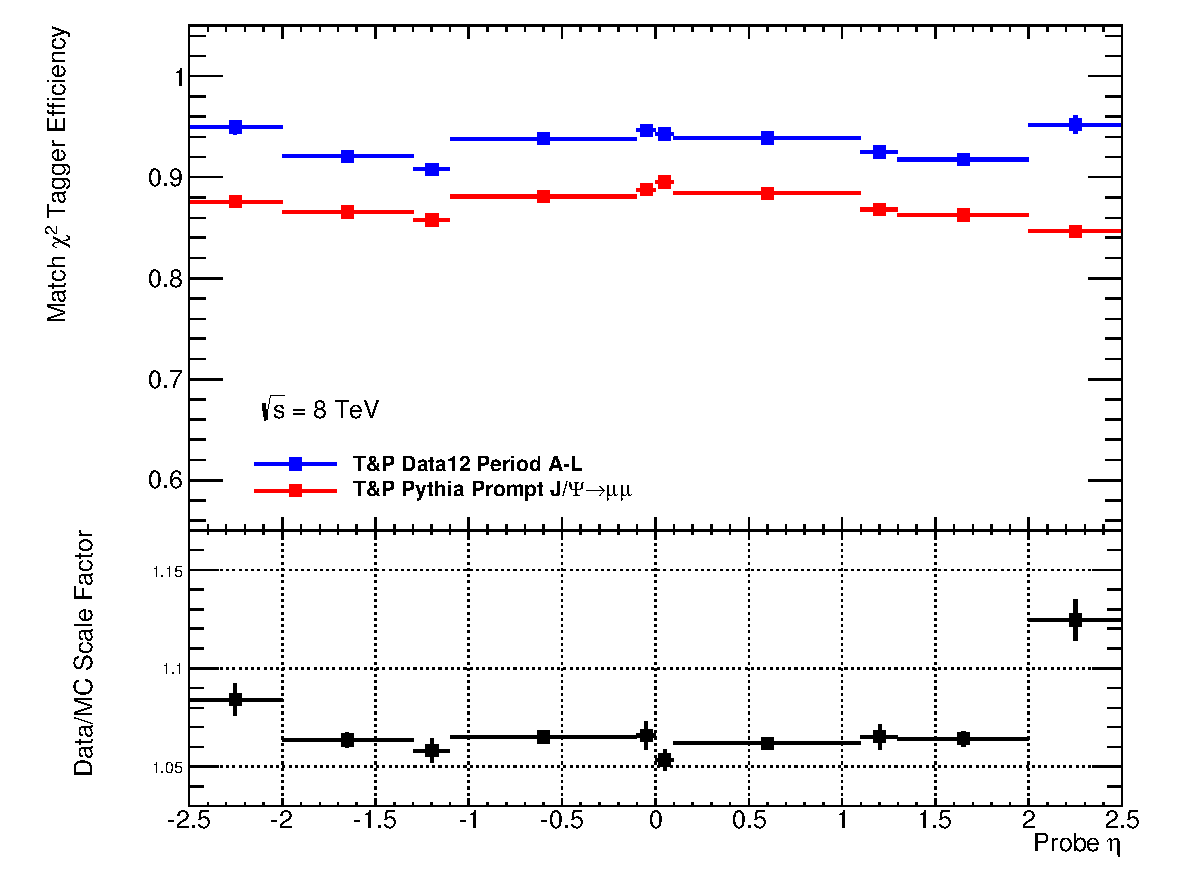
\includegraphics[width=\textwidth]{PartCalibration2012/Plots/SFPlots/eta_smt.pdf}
    \caption{\xsm\ efficiency and scale factor as a function $\eta$ of the probe muon} \label{fig:CalibrationEta}
  \end{subfigure}
  \caption{\xsm\ efficiencies and scale factor with respect to the angular position of the muon probe} \label{fig:label}
\end{figure}


